
%%%%%%%%%%%%%%%%%%%%%%%%%%%%%%%%
%------------------------------%
%%%%%%%%%%%%%%%%%%%%%%%%%%%%%%%%
\section{Introduction}
%%%%%%%%%%%%%%%%%%%%%%%%%%%%%%%%
%------------------------------%
%%%%%%%%%%%%%%%%%%%%%%%%%%%%%%%%

The objective of many genetic studies is to accurately identify variants associated with complex traits or diseases, and to estimate the effects of those variants. Such information is valuable for assessing an individual's risk of developing a particular condition, elucidating the underlying genetic architecture of a trait or disease, and identifying potential drug targets. However, this effort may be hindered by several factors such as non-independent samples, large numbers of variants, and linkage disequilibrium (LD). 

% \anna{keep this for later use when talking about genetic background?} Genetic variants are often correlated with each other such that univariate testing may be prone to false positives and biased estimates. When a genetic variant of interest is highly correlated with others, the effects of these will be attributed to the variant in question. This may result in causal SNPs being removed from analysis, so that only SNPs in LD with the causal loci, as opposed to the causal loci themselves, can be identified and their effects estimated. 

One method for analyzing data in the presence of correlated loci is LD pruning, which involves sequentially thinning SNPs, so that only those correlated with each other below some desired threshold are used in modeling and testing procedures. LD pruning can be an important preprocessing step in a GWAS analysis, for which there exist a variety of algorithms and methods. An alternative solution to the problem of LD is the use of multivariate methods such as multiple linear regression, which adjusts for and estimates the effects of numerous variants simultaneously. However, classical approaches rely on collecting data with more observations than unknown parameters. This is typically infeasible in genome-wide studies where the number of features greatly exceeds the number of observations. Penalized regression methods make such problems tractable by constraining the solution space of coefficient estimates. The Lasso is a widely used penalized regression method \citep{tibshirani1996regression}. It relies on an assumption of sparsity, which allows coefficient estimation and variable selection to be accomplished simultaneously. It also provides considerable computational advantages that scale up well to very large data sets. These features make the Lasso attractive for the analysis of high-dimensional genetic data where identifying a list of variants most highly associated with a particular trait is often of interest.

As with multiple linear regression models, Lasso penalized regression assumes independent observations and uncorrelated errors. In the presence of population structure or cryptic relatedness, however, samples are correlated, violating this assumption. If unaccounted for, this dependency can result in the identification of spurious associations. Though methods to correct for population stratification and cryptic relatedness have been extensively investigated, until recently the majority of this work has focused on plant and animal breeding data, much of which is experimentally controlled \citep{Amin2007, hoffman2013correcting, price2006principal, Rakitsch2012, bhatnagar2019simultaneous, Sillanpaeae2011}. While many standard correction techniques may in principal be applied to human genetic data, their performance has not been well-studied within the context of human ancestry and non-experimental conditions \citep{lawson2019population, barton2019population}.  

One reason that population stratification warrants such concern in genetic studies is that due to ethnic and geographic segregation, population stratification tends to be associated with differing environmental exposures and cultural practices \citep{thornton2015statistical, browning2011population}.  In other words, random genetic variation is likely to be correlated with non-genetic factors that also influence the trait of interest, thereby confounding the genotype-phenotype relationship and leading to spurious associations and biased estimates of SNP effects. Biased estimates of this nature severely hinder prediction and understanding differences among populations \citep{barton2019population}. Although bias at individual loci may be small, this bias becomes magnified when aggregated across thousands of SNPs, as is done when calculating polygenic risk scores \citep{barton2019population, peterson2019genome}.

In order to clarify and emphasize the importance of the subtle distinction between population structure and environmental heterogeneity, we present a detailed review of relevant concepts and methods. The remainder of this paper is organized as follows. In Section \ref{sec:background} we provide a summary of the causes and consequences of structure in the genetic data of seemingly unrelated individuals and formally define terminology used throughout this paper. We emphasize that confounding due to population structure, frequently cited as a driver of spurious associations, is a function of environmental heterogeneity, where genetic data serves as a proxy for differential environmental exposures \citep{Sillanpaeae2011, sul2018population, vilhjalmsson2012nature, barton2019population}. In so doing, we refine the definition of confounding due to population structure in terms of a non-genetic mechanism. In addition, we briefly review historical methods of correcting for population stratification and relatedness. In Section \ref{sec:methods} we provide a detailed review of the two most prevalent multivariate methods of adjusting for population stratification and relatedness at present: PCA adjusted Lasso penalized regression (PC-Lasso) and Lasso penalized multivariate LMMs (LMM-Lasso). We review the statistical details of how these methods attempt to correct for population structure and environmental heterogeneity. In Section \ref{sec:results}, we illustrate the concepts described in Section \ref{sec:methods} via simulation studies, where the data-generating mechanism formally differentiates between population structure and environmental heterogeneity. In addition, these results identify scenarios where particular methods may be most and least effective in accurately estimating the effect sizes of observed SNPs in the presence of unobserved confounding.




%%%%%%%%%%%%%%%%%%%%%%%%%%%%%%%%
%------------------------------%
%%%%%%%%%%%%%%%%%%%%%%%%%%%%%%%%
\section{Background} \label{sec:background}
%%%%%%%%%%%%%%%%%%%%%%%%%%%%%%%%
%------------------------------%
%%%%%%%%%%%%%%%%%%%%%%%%%%%%%%%%

%------------------------------%
\subsection{Structure in genetic data}

Population structure is defined by the existence of allele frequency differences that define sub-populations and is driven by the combined effects of evolutionary processes such as genetic drift, migration, demographic history, and natural selection \citep{gibson2015primer, tibayrenc2017genetics}. Population structure is broadly categorized based on whether it describes recent or ancient relatedness. Ancient relatedness describes the presence of a common ancestor many generations previously. The presence of distinct ancestry groups with different allele frequencies in a sample is known as \textbf{population stratification}. Recent relatedness describes the sharing of a common ancestor only several generations previously. Pedigree-based methods may be used to explicitly model recent relatedness if familial relationships are known. In the absence of known familial relationships, recent relatedness is referred to as \textbf{cryptic relatedness.} 

Population structure is a common phenomenon in genetic data. Varying levels of relatedness are almost always present among genetic samples, even in samples of unrelated individuals and seemingly homogeneous populations. For example, European American, Han Chinese, and most recently, cohorts within the UK Biobank data have been shown to exhibit patterns of population and geographic structure despite their seemingly similar subjects \citep{campbell2005demonstrating, xu2009genomic, chen2009genetic, haworth2019apparent}.

In this review we focus on methods to account for unobserved relatedness such as population stratification and cryptic relatedness. Throughout this paper, the terms \textbf{population structure} and \textbf{structured population} will be used to describe a sample of individuals in which population stratification, cryptic relatedness, or both are present. Population stratification in particular has been of great concern in genetic studies due to its potential to lead to spurious associations when population structure is associated with differences in both allele frequency and the trait or disease \citep{gibson2015primer}. This phenomenon is commonly described as \textbf{confounding due to population stratification}. The mechanism of this phenomenon warrants some discussion as it is often overlooked that population structure in and of itself does not confound the genotype-phenotype relationship. While population structure may directly affect observed allele frequencies, there must also exist some non-genetic mechanism by which population stratification affects the phenotype, namely, the environment \citep{barton2019population, vilhjalmsson2012nature}.


%------------------------------%
\subsection{Motivating example}

As an example, consider a genome wide association study (GWAS) to assess genetic variants associated with lung cancer in a sample comprised of subjects from two distinct subpopulations, A and B. Assume the minor allele of SNP $X$ is present with higher frequency in subpopulation A compared to subpopulation B, but has no direct effect on lung cancer. Also suppose these subpopulations are geographically segregated in a such a way that subpopulation A is exposed to good air quality, and subpopulation B to poor air quality, and that air quality does have a direct effect on lung cancer. A GWAS of data from these subpopulations would find SNP $X$ to be significantly associated with lung cancer. This spurious association is not identified because of the presence of population stratification itself, but because that stratification is related to a causal environmental exposure. Indeed, if subpopulations A and B were not subject to different air qualities, all else being equal, SNP $X$ would not be found to be associated with the phenotype.

% \anna{description of DAG below, in reference to previous one}

This mechanism of environmental confounding is summarized in the directed acyclic graph displayed in Figure \ref{fig:ps_env}. The undirected dashed line between population stratification and environmental exposure indicates that while we assume these elements are correlated, we do not assume any causal direction. Otherwise stated, we do not assume that environmental factors directly influence population-specific allele frequencies, or vice versa, only that the two may be related. In the context of our air quality example, this means that we assume air quality is not directly altering individuals' allele frequencies, nor are allele frequencies causing individuals to move to regions of better or worse air quality. Genetic relatedness and environmental effects may become associated over time for any number of complex reasons beyond the scope of this paper. However, as we will discuss, many methods of correcting for population structure rely on this relationship and do not formally differentiate between effects of population structure and those of environment. Such methods assume that genetic relatedness serves as an accurate proxy for environmental exposures, which may or may not be the case depending on the exposure and population in question.

\pb{Just an FYI, you may want not to call this diagram a ``Figure''.  Sometimes you're restricted in terms of the number of figures you can include, and this doesn't really need to be a figure, just a diagram (like an equation).  Same thing for the other DAG}

\begin{figure}[H]
\centering
\begin{tikzpicture}
    \node (1) at (0,0) {Population Stratification};
    \node (2) [right = of 1] {Environment};
    \node (3) [below = of 1] {Observbed SNPs};
    \node (4) [below = of 2] {Phenotype};
    \path[bidirected, -] (1) edge (2);
    \path (1) edge (3);
    \path (2) edge (4);
    \path (3) edge (4);
\end{tikzpicture}
\caption{Directed acyclic graph (DAG) of confounding due to population structure.}
\label{fig:ps_env}
\end{figure}

An additional source of confounding in genetic studies that we will briefly mention is that of confounding due to genetic background. This occurs in univariate association methods when a non-causal SNP is tested for association with a trait of interest, and that SNP is correlated with a causal SNP. As \citet{vilhjalmsson2012nature} note, any trait that has some genetic basis will be subject to genetic background effects, just as traits that are influenced by the environment may be subject to environmental confounding. Given the importance of both genetic and environmental contributions to many complex phenotypes, both genetic background and environmental confounding are important factors in our ability to identify true causal genetic relationships between SNPs and phenotype. LD pruning is commonly employed to reduce confounding due to genetic background in univariate association testing. However, we will focus on methods which address this via genomewide multivariate analysis.

%------------------------------%
\subsection{Correcting for population structure}

One of the first methods to address the problem of confounding due to population structure is the genomic control (GC) method. Because the effect of this confounding is to inflate the distribution of test statistics, GC introduces a factor to counteract this effect and restore the appropriate null distribution. This deflation factor is estimated using loci independent of the phenotype of interest and the loci being tested for association \citep{devlin1999genomic, bacanu2000power, wang2009testing}. However, quantifying the extent of inflation is not trivial, and is sensitive to the nature and quantity of the loci used to estimate it \citep{hellwege2017population, marchini2004effects}. Additionally, GC does not correct effect size estimates, so resulting coefficient estimates will be unreliable after GC is applied, even if their corresponding test statistics and p-values have been appropriately adjusted \citep{hellwege2017population}.

New statistical methods to control for the effects of confounding due to population stratification have proliferated as computational advances have allowed for the analysis of genetic data from large cohorts. Many of these methods attempt to block the causal pathway between population structure and observed SNP data. This is illustrated by the blocked arrow in Figure \ref{fig:ps_env_block}. As the figure shows, these methods do not directly address the environmental component of confounding due to population structure, instead controlling confounding by indirectly blocking the causal pathway between the environment and observed SNPs. 

\begin{figure}[H]
\centering
\begin{tikzpicture}
    \node (1) at (0,0) {Population Stratification};
    \node (2) [right = of 1] {Environment};
    \node (3) [below = of 1] {Observed SNPs};
    \node (4) [below = of 2] {Phenotype};
    \path[bidirected, -] (1) edge (2);
    \path[magenta, line width = 0.5] (1) edge (3);
    \path (2) edge (4);
    \path (3) edge (4);
    \tkzMarkSegment[color=magenta,pos=.5,mark=x](1,3)
\end{tikzpicture}
\caption{The causal pathway between the environment and observed SNPs may be indirectly blocked by many methods that attempt to reduce confounding due to population structure.}
\label{fig:ps_env_block}
\end{figure}

Whether or not such methods are effective at reducing confounding effects depends upon whether population structure can be accurately inferred. An important concept to note, and one that we will return to in Section \ref{sec:sim_env_conf}, is that population structure only leads to confounding if it is correlated with the environment.
In the presence of environmental heterogeneity which affects the phenotype of interest in a manner that is orthogonal to population structure, SNP-phenotype associations will not be confounded. This is due to the absence of a causal pathway between population stratification and environment, as depicted in Figure \ref{fig:ps_env_block2}. In such a scenario, failing to account for unobserved environmental effects is likely to result in greater variability, but SNP effect estimates will remain unbiased \citep{greenland1999causal}. We will return to this idea and its mathematical justification in Section \ref{sec:methods}. 

\begin{figure}[H]
\centering
\begin{tikzpicture}
    \node (1) at (0,0) {Population Stratification};
    \node (2) [right = of 1] {Environment};
    \node (3) [below = of 1] {Observed SNPs};
    \node (4) [below = of 2] {Phenotype};
    \path[bidirected, -, magenta] (1) edge (2);
    \path (1) edge (3);
    \path (2) edge (4);
    \path (3) edge (4);
    \tkzMarkSegment[color=magenta,pos=.5,mark=x](1,2)
\end{tikzpicture}
\caption{The causal pathway between the environment and observed SNPs may be blocked if genetic information does not serve as an accurate proxy for it.}
\label{fig:ps_env_block2}
\end{figure}

Assuming for now that population structure is correlated with environmental exposures and can be accurately inferred from available data, we return to our consideration of methods that attempt to control for confounding via the mechanism depicted in Figure \ref{fig:ps_env_block}. Such methods include LMMs, principal-component-based approaches, and stratified analyses. Stratified analyses refer to a general class of methods which attempt to infer subject membership within a discrete number of nonoverlapping subpopulations. Subsequent analyses are conducted within each subpopulation, and the subpopulation-specific results may then be combined via meta-analysis \citep{pritchard1999use, pritchard2000association}. By partitioning the overall sample size in this manner, the structured association method is vulnerable to a loss of power. Additionally, it relies on the assumption that these subpopulations are distinct and nonoveralapping. This assumption may not accurately reflect the characteristics of a particular sample, such as one consisting of admixed populations, or recent relatedness. Considered in the context of our air quality example, rather than the existence of two subpopulations with exposure to either good or bad air quality, there may also be individuals who fall between these two extremes and are characterized by continuously varying relatedness and a gradient of air quality. By clustering those individuals within in one subpopulation or another, we lose information about relatedness by oversimplifying the population structure.

A different approach is to create an approximation of population structure using surrogate variables, and to adjust for these as an additional model covariates. Principal component-adjustment (PC-adjustment) methods use the first several left singular vectors of a pairwise similarity matrix as these surrogate variables \citep{price2006principal}. This approach may be used in univariate or multivariate frameworks, and allows for analysis on the entirety of a structured sample. 

% rely on a pair-wise similarity matrix
Like PC-adjustment methods, LMMs utilize the left singular vectors of a similarity matrix to estimate and subsequently correct for relatedness among subjects. In an LMM, however, these left singular vectors are treated as random, rather than fixed effects. The term LMM has been used to describe a number of distinct but related procedures for analyzing structured genetic data which differ in their objectives and methods. There are two main objectives of LMMs used in a structured genetic context: estimating narrow-sense heritability, and estimating individual SNP effects.

Among LMM methods that aim to estimate heritability, the most well-known example is genome-wide complex trait analysis (GCTA) \citep{yang2011gcta}. In this framework, all observed SNPs are treated as random effects. These effects are integrated out in order to estimate a genetic variance component, which in turn, is used to quantify the total narrow-sense heritability of a trait \citep{yang2010common}.

LMMs can also be used to estimate SNP effects, and this can be done in either a univariate or multivariate manner. Univariate approaches attempt to estimate the marginal effect of a SNP on the phenotype and assess the statistical significance of SNP-phenotype associations while controlling for population structure by modeling it as a random effect using a genetic similarity matrix \citep{yu2006unified, kang2010variance, kang2008efficient}. However, as with all univariate testing approaches, univariate LMM implementations are prone to spurious associations and biased effect estimates in the presence of LD. 

Multivariate mixed model approaches reduce these problems by modeling the relationship between a phenotype of interest and all SNPs simultaneously via penalized regression, while correcting for dependencies among subjects \citep{Rakitsch2012, bhatnagar2019simultaneous}. This approach assumes there are a relatively small number of SNPs associated with the phenotype of interest that have large effect sizes. These SNPs will be included in the model as both fixed and random effects, while SNPs with smaller effect sizes are modeled only as part of the random effect in order to control for dependent errors due to relatedness and sample structure. 

The remainder of this review will focus on the performance of such multivariate Lasso-penalized methods for the analysis of continuous, normally distributed outcomes. Specifically, PC-adjustment and LMM methods, which we will refer to as PC-Lasso and LMM-Lasso, respectively. We consider two similar implementations of the LMM-Lasso method, one developed by \citet{Rakitsch2012} and a more recent implementation from \citet{bhatnagar2019simultaneous}. Subsequent references to LMM-Lasso apply to both implementations, unless otherwise stated. Where necessary, we will differentiate between these implementations by referring to them as LMM-Lasso-Rakitsch and LMM-Lasso-ggmix, respectively. 

Several studies have shown that LMMs outperform PC-adjustment methods in the univariate framework \citep{wang2013analytical, kang2010variance, zhao2007arabidopsis}. However, to the best of our knowledge this is the only comprehensive review and comparison of these methods in a penalized multivariate framework and using a simulation scheme motivated by human genetic relatedness and the environmental mechanism of confounding due to population structure.\\

%%%%%%%%%%%%%%%%%%%%%%%%%%%%%%%%
%------------------------------%
%%%%%%%%%%%%%%%%%%%%%%%%%%%%%%%%
\section{Methods} \label{sec:methods}
%%%%%%%%%%%%%%%%%%%%%%%%%%%%%%%%
%------------------------------%
%%%%%%%%%%%%%%%%%%%%%%%%%%%%%%%%



%------------------------------%
\subsection{LMM and PC models}

To describe and compare PC-Lasso and LMM-Lasso, we consider an $n \times p$ matrix of genotype data $\bG$ for $n$ subjects and $p$ SNPs, where each $G_{ij} \in \{ 0, 1, 2 \}$ enumerates the number of allele copies subject $i$ has for SNP $j$. In order to equitably compare SNP effects, regardless of allele frequency, in practice $\bG$ is standardized. We denote the standardized version of this genotype matrix as $\bX$, where each $X_{ij} = (G_{ij} - 2 \pi_j) / \sqrt{\pi_j (1 - \pi_j)}$ and $\pi_j$ is the minor allele frequency (MAF) of SNP $j$ \citep{zhang2015principal, price2006principal}. Additionally, $\bX_0$ represents an $n \times p_0$ matrix of unpenalized covariates and the intercept. Thus, at a minimum, $\bX_0$ will be an $n \times 1$ vector of 1s to represent the intercept, in which case $\bbeta_0 \equiv \beta_0$ is the scalar intercept. However, $\bX_0$ may additionally include observed covariates such as age, sex, or smoking history, which are included in the model without penalty. We assume that the $n \times 1$ vector of continuous phenotype values, $\by$, can be expressed as the sum of these covariates, additive SNP effects, environmental effects, and observational noise, and consider the linear model,
\begin{equation}
    \label{eqn:model}
    \by = \bX_0 \bbeta_0 + \bX\bbeta + \bZ\bgamma + \beps
\end{equation}
where $\bbeta_0$ is a $p_0 \times 1$ vector which includes the intercept term and the effects of any unpenalized covariates, $\bbeta$ is a $p \times 1$ vector of SNP effects, $\bgamma$ is a $q \times 1$ vector of environmental effects, $\bZ$ is an $n \times q$ matrix that allocates environmental effects among subjects, and $\beps \sim N(\boldsymbol{0}, \sigmaee \bI_n)$. Often it is assumed that subjects belong to $q \le p$ subpopulations, and $\bZ$ is a corresponding incidence matrix of 0s and 1s. However, as we will discuss, this is not the only possibility.

A key feature which differentiates \eqref{eqn:model} from traditional linear mixed models is that in our setting, $\bZ$ is not observed directly, although we still wish to correct for it in order to remove the effects of confounding influences. A common convention is to assume $\bZ = \bX$ \citep{wang2018multiplex, lippert2011fast, yang2014advantages}; we will discuss the rationale for this approach in Section~\ref{sec:sim_env_conf}.  This, in turn, motivates the methods by which LMM-Lasso and PC-Lasso attempt to model unobserved confounding effects using observed genetic data.

Both PC-Lasso and LMM-Lasso rely on matrix decompositions of $\bX$ and the realized relationship matrix (RRM), $\bK = p^{-1} \bX \bX^\T$, which describes the pair-wise genetic similarity among subjects \citep{hayes2009increased}. Using the singular value decomposition (SVD) of the standardized genotype matrix, we can derive the spectral decomposition of the RRM: 

\begin{equation}
    \label{eqn:k}
    \bK = \frac{1}{p} \bX \bX^\T = \frac{1}{p} \bU \bD^2 \bU^\T = \frac{1}{p} \bR \bR^\T,
\end{equation}
where $\bD^2$ is an $n \times n$ diagonal matrix containing the $k$ nonzero eigenvalues of $\bK$ on the top-left diagonal, followed by $n - k$ zeroes on the bottom-right diagonal. $\bU$ is the corresponding $n \times n$ orthonormal matrix of left eigenvectors, or principal components, of $\bK$. The first $k$ columns of $\bU$ correspond to the nonzero eigenvalues of $\bK$, and the columns of $\bR$ are thus the principal components of $\bK$ weighted by their corresponding singular values. 

%------------------------------%
\subsection{PC-Lasso}
PC-Lasso uses the first $k$ principal components of $\bK$ to approximate $\bZ\bgamma$ and includes them in the model as unpenalized covariates. This corresponds to the regression model
\begin{equation}
    \label{eqn:pca_reg}
    \by = \bX_0\bbeta_0 + \bX\bbeta + \bU_{1:k}\boldsymbol{\alpha} + \beps 
\end{equation}
$$ \beps \sim N(\boldsymbol{0}, \sigmaee \bI), $$
where $\bU_{1:k}$ is the $n \times k$ matrix of principal component vectors, $\boldsymbol{\alpha}$ their corresponding $k \times 1$ coefficient vector, and all other parameters are as defined in equation \eqref{eqn:model}. In a penalized regression framework, this model yields the objective function
\begin{equation}
    \label{eqn:pca_obj}
    Q(\bbeta, \boldsymbol{\alpha}|\bX, \by) = \frac{1}{2n} ||\by - \bX_0\bbeta_0 - \bX \bbeta- \bU_{1:k}\boldsymbol{\alpha}||_2^2 + \lambda || \bbeta ||_1
\end{equation}
where $\lambda$ is a tuning parameter, and $|| \boldsymbol{\beta} ||_1 = \sum_{j=1}^p |\beta_j|$ denotes the $\ell_1$ norm of the regression coefficients, and $||\mathbf{x}||_2 = \sqrt{\sum_{i=1}^p x_i^2}$ the $\ell_2$ norm. Note that the principal component regression coefficients, $\boldsymbol{\alpha}$, are not included in the penalty term. 

%------------------------------%
\subsection{LMM-Lasso}
\label{sec:lmmlasso}

Conversely, LMM-Lasso models $\bZ\bgamma$ as a random effect, which corresponds to the LMM model
\begin{equation}
    \label{eqn:lmm_reg}
    \by = \bX_0\bbeta_0 + \bX\bbeta + \bX\bgamma+ \beps,
\end{equation}
$$ \beps \sim N(\boldsymbol{0}, \sigmaee \bI) $$
$$ \bgamma \sim N(\boldsymbol{0}, p^{-1} \sigmagg \bI) \Rightarrow \bX \bgamma \sim N(\boldsymbol{0}, \sigmagg \bK), $$
where $\sigmagg$ is the additive genetic variance, and we assume $\beps \independent \bgamma$. Rather than assuming anything about $\bgamma$ directly, a common representation paramaterizes the model in terms of $\bu=\bX\bgamma$, which yields an equivalent model. 

We will first derive the LMM-Lasso objective function in the absence of unpenalized covariates for the sake of notational simplicity. Following equation \eqref{eqn:lmm_reg}, in the absence of unpenalized covariates the LMM assumes $\by \sim N(\bX \bbeta, \bV)$, where $\bV = \sigmagg \textbf{K} + \sigmaee \textbf{I}$. LMM-Lasso uses the covariance structure of the errors and properties of the multivariate normal distribution to transform the original data and diagonalize the errors in a manner akin to generlized least squares (GLS). Specifically, left-multiplying the original data by $\bV^{-1/2}$ yields 

\begin{equation}
\label{eqn:rtY_distn}
\bV^{-\frac{1}{2}}\by \sim N(\bV^{-\frac{1}{2}} \bX \bbeta, \bI),
\end{equation}
and thus an ordinary Lasso model can be fit on the transformed data, ($\bV^{-\frac{1}{2}}\bX, \bV^{-\frac{1}{2}}\by$). 

Using the spectral decomposition of $\bK$ described in equation \eqref{eqn:k}, we can gain further insight into the mechanism of this transformation. Note that $\bV^{-1}$ can be expressed using the following matrix factorization 
\begin{align*}
    \bV^{-1} &= (\sigmagg \bK + \sigmaee \bI)^{-1}\\
    &=(\sigmagg \bU \bD^2 \bU^\T + \sigmaee \bU \bU^\T)^{-1}\\
    &= (\bU (\sigmagg \bD^2 + \sigmaee \bI) \bU^\T)^{-1}\\
    &=\bU (\sigmagg \bD^2 + \sigmaee \bI)^{-1} \bU^\T\\
    &=\bU \bW^2 \bU^\T.
\end{align*}
By incorporating these decompositions, the transformed data can be expressed as $\bW \bXT$ and $\bW \byT$, respectively, where $\bXT = \bU^\T \bX$, $\byT = \bU^\T \by$, $\bW = \text{diag}\{w_1, ... w_n\}$, and $w_i$ corresponds to the square root of the $i$th element of the diagonal matrix $(\sigmagg \bD^2 + \sigmaee \bI)^{-1}$. Together, this yields the objective function
\begin{equation}
\label{eqn:lmm_obj}
Q(\bbeta | \bXT, \byT, \bW) = || \bW (\byT - \bXT \bbeta)||_2^2 + \lambda || \bbeta ||_1.
\end{equation}
In the presence of an intercept and unpenalized covariates, \eqref{eqn:rtY_distn} becomes 
\begin{equation}
\bV^{-\frac{1}{2}}\by \sim N\left(\bV^{-\frac{1}{2}} \bX{^\prime} \bbeta{^\prime}, \bI \right),
\end{equation}
where $\bX{^\prime} = \begin{bmatrix} \bX_0 & \bX \end{bmatrix}$ and $\bbeta{^\prime} = \begin{bmatrix} \bbeta_0^\T & \bbeta^\T \end{bmatrix}^\T$. This in turn leads the objective function
\begin{equation}
Q(\bbeta | \bXT{^\prime}, \byT, \bW) = || \bW (\byT - \bXT{^\prime} \bbeta{^\prime})||_2^2 + \lambda || \bbeta ||_1,
\end{equation}
where $\bXT{^\prime} = \bU^\T \bX{^\prime}$, so that all of the data are transformed, but only the elements of $\bbeta{^\prime}$ corresponing to SNPs are penalized. 

%------------------------------%

Different variance component estimation methods lead to different forms of $\widehat{\bW}$ and two distinct LMM-Lasso variants: LMM-Lasso-Rakitsch and LMM-Lasso-ggmix. LMM-Lasso-Rakitsch uses a two-step procedure for estimating the variance components, $\sigmaee$ and $\delta := \sigmaee / \sigmagg$ \citep{Rakitsch2012}. These variance components and the corresponding weights are estimated once under the assumption of a null model. A Lasso model can then be fit on the transformed data to estimate $\boldsymbol{\beta}$ using standard software for coordinate descent, such as \texttt{glmnet} \citep{glmnet} or \texttt{ncvreg} \citep{ncvreg}. LMM-Lasso-ggmix iteratively updates $\widehat{\boldsymbol{\beta}}$ and the variance components via a block coordinate descent algorithm \citep{bhatnagar2019simultaneous}. This iterative update scheme prevents the use of standard Lasso software, but is implemented in the \texttt{R} package \texttt{ggmix} \citep{ggmix}. We further discuss differences between these methods in Section \ref{sec:results}.

%------------------------------%
% \subsubsection{\anna{Intuition from GLS (?) p-values and SEs in response to rotation?}}


%------------------------------%
\subsection{Relationship between PC-Lasso and LMM-Lasso}

It has been shown that the random effect formulation of model \eqref{eqn:model} used by LMM-Lasso can be equivalently expressed in terms of fixed effects in the absence of penalization?. \citet{zhang2015principal} derived this equivalence using a probabilistic PCA formulation, while \citet{hoffman2013correcting} used the singular value decomposition of $\bX$, which we briefly review.

Using the result of the decomposition from \eqref{eqn:k}, $\bK = p^{-1} \bR \bR^\T$ , the LMM model \eqref{eqn:lmm_reg} can be written equivalently as

\begin{equation}
    \label{eqn:pc_lmm_equiv}
    \by = \bX_0 \bbeta_0 + \bX \bbeta + \bR \bgamma + \beps
\end{equation}

$$ \beps \sim N(\boldsymbol{0}, \sigmaee \bI) $$
$$ \bgamma \sim N(\boldsymbol{0}, p^{-1} \sigmagg \bI) \Rightarrow \bR \bgamma \sim N(\boldsymbol{0}, \sigmagg \bK).$$
Based on the relationship between equations \eqref{eqn:pca_reg} and \eqref{eqn:pc_lmm_equiv}, we can see that modeling the principal components of $\bK$ as fixed or random effects relies on the same underlying regression model. However, while the LMM includes all the principal components, only $k < n$ are included in the fixed effects model. 

Additionally, while the fixed effects model considers the principal components $\bU$ of $\bK$, the LMM considers the principal components weighted by their corresponding eigenvalues. The eigenvalues have been shown to serve as a measure of biological relevance of each principal component in relation to underlying population structure \citep{hoffman2013correcting, price2006principal}. 

From a Bayesian perspective, using the first $k$ principal components as regression covariates can be viewed as assigning uniform priors to the first $k$ components of $\bgamma$, while the remaining $n - k$ components receive a prior with unit mass at zero. These assignments imply certainty that the effect of population structure on the phenotype is fully captured by the first $k$ PCs. In contrast, the LMM approach can be viewed as assigning a Gaussian prior on each component of $\bgamma$, with variances proportional to the corresponding eigenvalues \citep{astle2009population}. 

Whether modeled as a fixed or random effect, the underlying effect of $\bZ \bgamma$ on phenotype remains the same, but its treatment as a fixed or random effect has important implications in terms of model fitting and estimation. Modeling unobserved confounding using fixed effects requires estimation of $p_0 + p + k$ parameters, compared to the $p_0 + p + 2$ required of an LMM, which may result in a loss of power \citep{zhang2015principal}. Additionally, when modeling $\bZ \bgamma$ using fixed effects, determining the appropriate number of principal components, $k$, to adjust for is non-trivial, and has been the subject of numerous studies \citep{patterson2006population, zhao2018practical}. It has been shown that including too many or too few principal components can result in power loss or increased Type I errors, respectively \citep{zhang2015principal}. Nevertheless, a common practice is to include the ten largest principal components in the analysis \citep{zhao2018practical}. This is the approach we take when implementing PC-Lasso in Section \ref{sec:results}.


%------------------------------%
\subsection{Partitioning the effects of environmental confounding}
\label{sec:sim_env_conf}

In carrying out simulation studies of the LMM regression model \eqref{eqn:lmm_reg}, a common practice is to draw a new value of the quantity $\bX\bgamma$ from a $N(\boldsymbol{0}, \sigmagg \bK)$ for each replication of the analysis \citep{Rakitsch2012, bhatnagar2019simultaneous}.  We argue that this is somewhat misleading from the perspective of understanding the statistical properties of the method in the presence of environmental heterogeneity. Averaging over situations in which the environmental confounding is constantly changing direction and magnitude has the effect of ``washing out'' bias in $\bbetaHat$. 

Consider our earlier example involving confounding due to air quality. Simulating $\bgamma$ as a random quantity for each replication corresponds to subpopulation A being exposed to good air quality in one replication, and bad air quality in the next. Reporting the average across these situations is inconsistent with the question we are truly interested in, namely: what would happen if we took repeated samples from populations A and B, when these populations are subject to different environmental exposures? Those repeated samples would show a systematic bias due to the difference in air quality, but this is masked if $\bgamma$ is assumed to be random. Treating $\bgamma$ as a fixed quantity so that environmental effects are consistent across replications more closely approximates environmental confounding.



To illustrate this concept mathematically, consider the low-dimensional ordinary least squares (OLS) estimates of $\bbeta$ based on model \eqref{eqn:lmm_reg} where, without loss of generatlity, we assume $\bX_0 \bbeta_0 = \boldsymbol{0}$ for ease of notation: 
\begin{align}
    \mathbb{E}(\bbetaHat) &= (\bX^\T \bX)^{-1} \bX^\T \mathbb{E}(\by) \notag \\
    &=  (\bX^\T \bX)^{-1} \bX^\T \mathbb{E}(\bX\bbeta + \bX\bgamma + \beps) \label{eqn:expectation}\\
    &\quad \notag\\
    \mathbb{V}(\bbetaHat) &= (\bX^\T \bX)^{-1} \bX^\T \mathbb{V}(\by) \notag\\
    &=  (\bX^\T \bX)^{-1} \bX^\T \mathbb{V}(\bX\bbeta + \bX\bgamma + \beps) \notag\\
    &=  (\bX^\T \bX)^{-1} \bX^\T \mathbb{V}(\bX\bgamma + \beps) \bX  (\bX^\T \bX)^{-1} \label{eqn:variance}.
\end{align}
Under the assumption that environmental effects arise from a random process, $\bgamma \sim N(\boldsymbol{0}, p^{-1} \sigmagg \bI)$, equations \eqref{eqn:expectation} and \eqref{eqn:variance} yield $\mathbb{E}(\bbetaHat) = \bbeta$, and $\mathbb{V}(\bbetaHat) = p^{-1}\sigmagg\bI + \sigmaee (\bX^\T \bX)^{-1}$, respectively. However, under the assumption that the quantity $\bgamma$ is fixed, equations \eqref{eqn:expectation} and \eqref{eqn:variance} yield $\mathbb{E}(\bbetaHat) = \bbeta + \bgamma, \mathbb{V}(\bbetaHat) = \sigmaee (\bX^\T \bX)^{-1}$, allowing us to quantify estimation bias due to environmental heterogeneity. 

Although we derive these quantities under model \eqref{eqn:lmm_reg}, where $\bZ = \bX$, these results also hold for the more general model \eqref{eqn:model}, where $\bZ \ne \bX$. We see this by decomposing $\bZ \bgamma$ into components in and orthogonal to the column space of the projection matrix of $\bX$.  Let $\boldsymbol{P}_{\bX} = \bX (\bX^\T \bX)^{-1} \bX^\T$ denote the projection matrix of $\bX$, with $\mathcal{C}(\boldsymbol{P}_{\bX})$ and $\mathcal{N}(\boldsymbol{P}_{\bX})$ denoting the column and null spaces of $\boldsymbol{P}_{\bX}$, respectively. Then there exist $\boldsymbol{\tau}, \boldsymbol{\psi}: \bZ \bgamma = \bX \boldsymbol{\tau + \psi}$, where $\bX \boldsymbol{\tau} \in \mathcal{C}(\boldsymbol{P}_{\bX})$ and $\boldsymbol{\psi} \in \mathcal{N}(\boldsymbol{P}_{\bX})$.  This in turn means that
\begin{align}
    \label{eqn:partition_e}    \by &= \bX\bbeta + \bZ\bgamma + \beps \notag \\
    &= \bX\bbeta + \bX \boldsymbol{\tau} + \boldsymbol{\psi} + \beps \notag\\
    &=  \bX \bbeta{^*} + \beps{^*};
\end{align}
note that $\boldsymbol{\tau}$ quantifies bias in the estimated $\bbetaHat^*$ and $\boldsymbol{\psi}$ is absorbed by the residual error term. In other words, any model specified in terms of $\bZ$ and $\bgamma$ is equivalent to a parameterization using $\bX$ and $\boldsymbol{\tau}$.  This result provides the explicit mathematical justification for our statement from Section \ref{sec:background}, that SNP-phenotype associations will be unbiased in the presence of environmental heterogeneity which does not correspond to population structure.

Furthermore, the proportion of the environmental effect in the column space of $\boldsymbol{P}_{\bX}$ (i.e., the portion that will cause confounding) is given by
\begin{equation}
    \label{eqn:ratio}
    \text{CP} = ||\bX \boldsymbol{\tau}||_2^2 / ||\bZ \bgamma||_2^2,
\end{equation}
which we refer to as the Confounding Proportion (CP). The CP can range from 0 (no confounding) to 1 (entirely confounded). In the extreme case where $\bZ \bgamma$ is completely independent of population structure, $\bZ \bgamma \in \mathcal{N}(\boldsymbol{P}_{\bX})$ and $\bX \boldsymbol{\tau} = \boldsymbol{0}$ so that $\mathbb{E}(\bbetaHat^*) = \bbeta$. In this scenario, the SNP-phenotype associations will be unbiased, but the residual error will be inflated. 

In real data settings CP cannot be calculated since $\bZ \bgamma$ is not directly observed. In simulation settings, however, this ratio is a useful metric for quantifying the degree to which $\bZ \bgamma$ reflects population structure and has the potential to bias SNP-phenotype associations. We will use CP in our interpretation of the simulation results in Section \ref{sec:results}. Given the high-dimensional nature of our data, we use a low-rank approximation of $(\bX^\T \bX)^{-1}$ in order to ensure a unique solution.

%------------------------------%
\subsection{Simulation study}
%------------------------------%

\subsubsection{Generation of synthetic phenotypes}

Given the nature of environmental confounding in our setting of interest, and in order to assess methodological performance in terms of estimation accuracy and bias, we simulate from the data-generating model
\begin{equation}
    \label{eqn:sim}
    \by = a \bX \bbeta + b \bZ \bgamma + c \beps,
\end{equation}
where $\by$ represents the synthetic phenotype, $\bgamma$ is a fixed quantity (see Section~\ref{sec:sim_env_conf}), and $a, b, c$ are scaling factors determined such that the variance of $\by$ is equal to 1 and is partitioned into genetic signal, environmental confounding, and random noise components,
\begin{equation}
    \label{eqn:parition_y}
    \mathbb{V}(\by) = \eta + (1 - \eta) \xi + (1-\eta)(1-\xi).
\end{equation}
$\eta$ defines the proportion of the variance of $\by$ attributable to additive genetic factors, commonly referred to as the narrow-sense heritability, $h^2 = \sigmagg/(\sigmagg + \sigmaee)$. The parameter $\eta$ also describes the data-generating model's signal to noise ratio (SNR), while $\xi$ partitions the remaining variance of $\by$ into latent environmental heterogeneity and random noise. So, for example $\eta = 0.5$ and $\xi = 0.8$ corresponds to a 1:1 SNR, and means that 50\% of the variability in $\by$ is due to additive genetic effects, and 40\% due to unobserved environmental effects. 

\subsubsection{SNP matrix generation}

We generated these synthetic phenotypes using three types of high-dimensional ($p > n$) $\bG$ matrices, which were then standardized to yield the corresponding $\bX$ matrix: (1) simulated SNP data from admixed subpopulations, (2) simulated SNP data from independent subpopulations, and (3) real genome-wide SNP data from known caucasian ($n = 417$), African American ($n = 134$), and Hispanic ($n = 37$) subpopulations \citep{larkin2015objectives}. We refer to these as the 1D Linear Admixture, Independent Subpopulations, and Empirical data, respectively. For all data types $p = 1000$ with 50 causal SNPs. For the simulated 1D Linear Admixture and Independent Subpopulations data $n = \{200, 400, 600, 800 \}$, and $n = 588$ for the Empirical data. 


\subsubsection{Subpopulation structure}
\label{sec:subpopulation_structure}
For the fully simulated data, two subpopulation structures were considered, which we refer to as ``fine'' and ``coarse''.  We define a coarse structure to be one characterized by a few large subpopulations intended to model large-scale environmental heterogeneity and population stratification, such as that described in our motivating air quaility example. Conversely, we define a fine subpopulation structure to be one characterized by many small subpopulations, representing a continuum of environmental heterogeneity. Whether fine or coarse, the simulated data were generated such that subpopulations (also known as founding populations) are of equal size. We note that the distinction between fine and coarse structure is an entirely different concept than the level of admixture in the simulated data. It is the size of the subpopulations, not the level of admixture, that determines what we refer to as fine or coarse structure. For example, both the Independent Subpopulation and 1D Linear Admixture simulated data may be comprised of fine or coarse structure. However, the subpopulations will be more distinct in the unadmixed Independent Subpopulation data than in the 1D Linear Admixed data. The Empirical data is comprised of three racial subpopulations; one relatively large, one small, and one in the middle. Thus it represents a hybrid of our simulated coarse and fine structures, with little apparent admixture. Supplementary Figures \ref{fig:admixed} - \ref{fig:empirical} illustrate the simulated kinship structures, as well as that for the Empirical SNP data. 

\subsubsection{Patterns of environmental effects}

For each $\bX$ matrix, $\bZ$ was a corresponding incidence matrix of 1s and 0s identifying subpopulation, or founding population membership, which assigns the corresponding environmental effect found in $\bgamma$. Various $\bgamma$ patterns were considered in order to investigate the effects of distinct forms of environmental confounding. Our initial hypothesis was that simple patterns of environmental effects could be well-approximated by a linear combination of the observed genetic data and well-corrected for by both PC-Lasso and LMM-Lasso, while PC-Lasso would be unable to represent and correct for more complex patterns of environmental effects.

Environmental effects may be complex in different ways. Firstly, we considered whether individuals in genetically similar subpopulations would experience similar environmental effects. For example, a geographic environmental exposure such as the air quality described in our motivating example is likely to be similar among genetically related individuals due to concordance between genetic clusters and geography. However, behavior-based environmental exposures may be less likely to be shared by subpopulations which are genetically and geographically similar. As an example, \citet{ng2014smoking} found considerable within-region variation in smoking rates in Africa, Asia, and South America. We refer to environmental effects that are similar among genetically similar subpopulations as concordant, and to those that are not as discordant. Secondly, we considered two patterns of environmental effect sizes, which we refer to as exponential and dichotomous. We use the term dichotomous to describe two effect sizes each experienced by half of the population, regardless of the number of subpopulations. While exponential effects refer to a unique effect size for each subpopulation with exponentially increasing magnitudes. 

 To evaluate the performance of penalized LMM methods in the presence of these different forms of confounding complexity, we consider environmental effects which are concordant or discordant in nature in the presence of both exponential and dichotomous effect sizes, for a total of four distinct $\bgamma$ patterns. Figure \ref{fig:gamma_structures} provides a visual summary of the four coefficient patterns, where the subpopulations on the x-axis are ordered by genetic similarity so that subpopulation 1 is most genetically similar to subpopulation 2, and least similar to subpopulation 10. This may also be thought of as subpopulations ordered spatially along a 1-dimensional geographic region.
\begin{figure}[H]
    \centering
    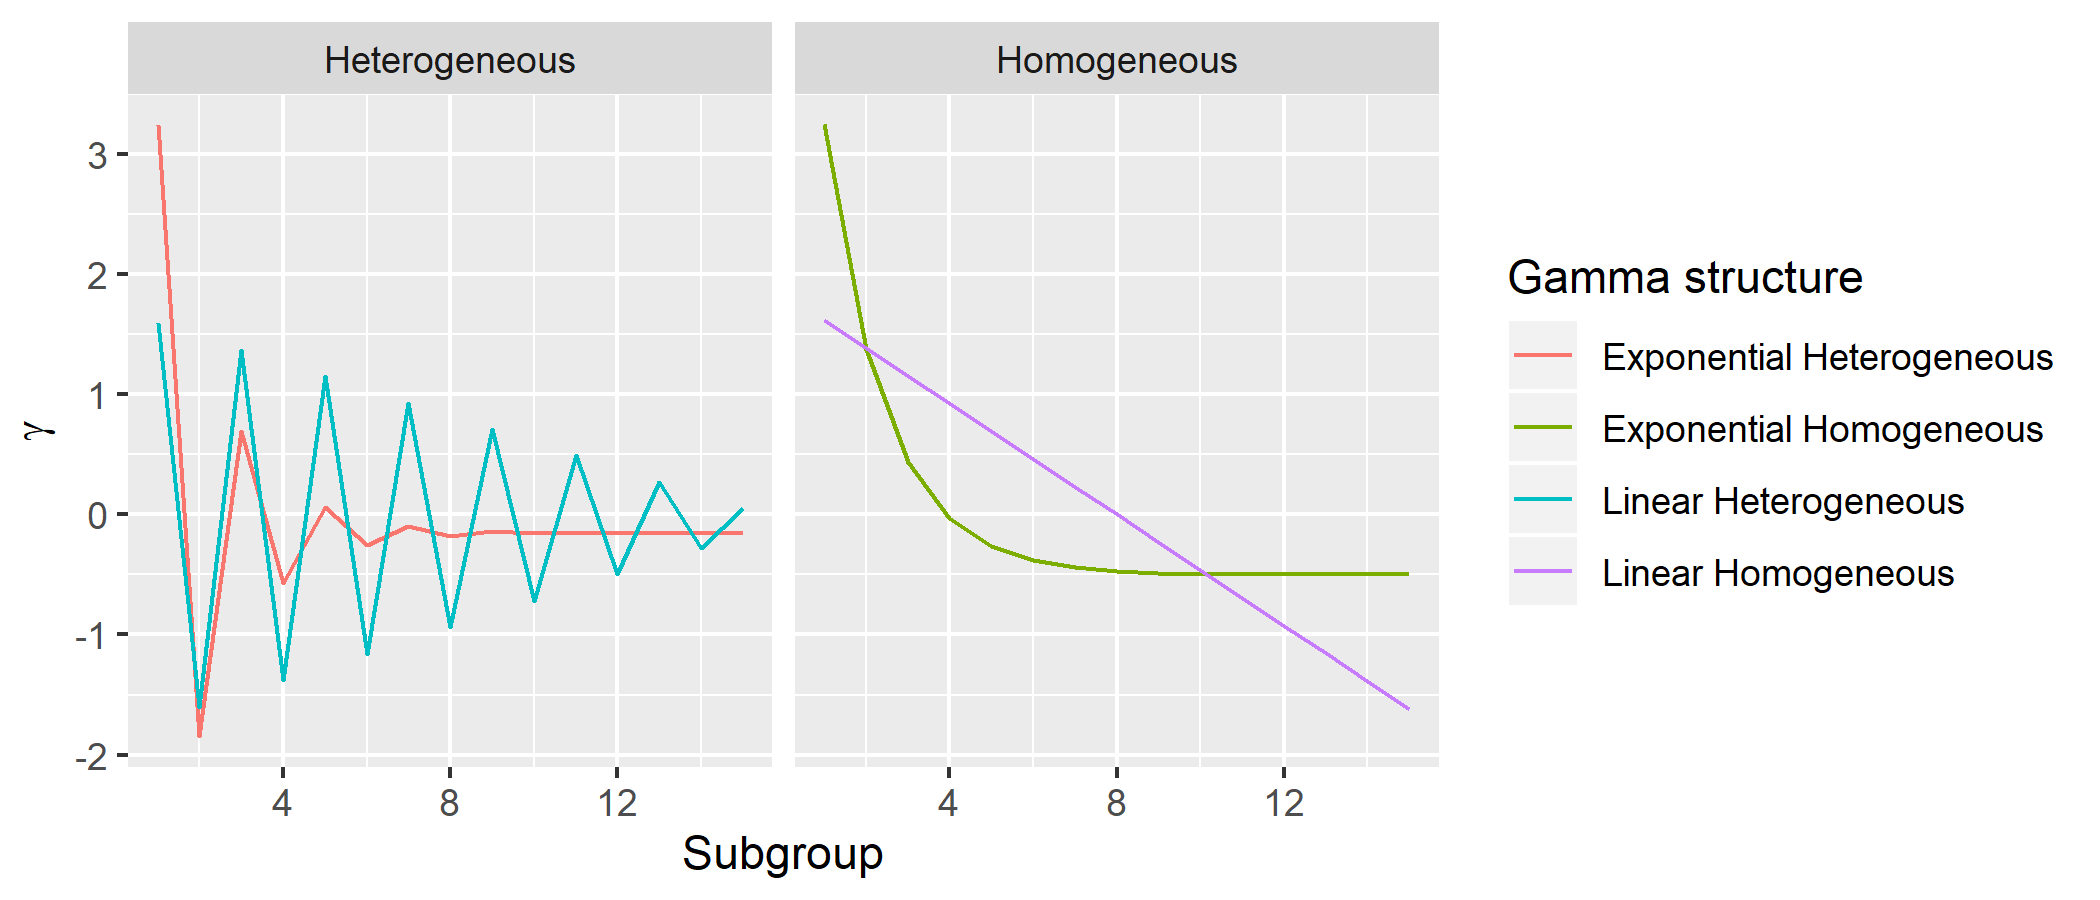
\includegraphics[scale = 0.9]{figures/gamma_structure.png}
    \caption{An illustration of four distinct patterns of environmental effects and corresponding $\bgamma$ values in the presence of 10 subpopulations ordered by genetic similarity.}
    \label{fig:gamma_structures}
\end{figure}
\noindent In the case of concordant and dichotomous effects, Figure \ref{fig:gamma_structures} shows that the first five ordered subpopulations are subject to an effect size of 1, while the second five are subject to an effect size of $-$1. In the case of discordant dichotomous effects, all subpopulations again experience an effect size with an absolute value of 1, however, the directions of these effects alternate among the ordered subpopulations so that genetically similar subpopulations do not experience similar environmental effects. 

\subsubsection{Tuning parameter selection}
Selection of the tuning parameter $\lambda$ plays an important role in all penalized regression methods, with many possible approaches. Here, for each model, we selected the $\lam$ value such that 50 SNPs were selected (recall that 50 is also the true number of causal SNPs). This method for selecting $\lambda$ was chosen in an attempt to compare the performance of all methods fairly, and as a strategy to evaluate methods in terms of variable selection, as it allows for direct comparison of the first 50 variables each method lets into the model.

Although cross-validation and information criterion-based methods are commonly used to select $\lambda$ values, in this context they have the potential to result in misleading comparisons across methods. Cross-validation may be inadvisable for LMMs, and in the presence of samples with underlying structure, as is the case here \citep{roberts2017cross}. While information criterion methods such as BIC present another option for selecting $\lambda$, they may be unstable in high dimensions. In addition, because Lasso, PC-Lasso, and LMM-Lasso use different likelihoods, an information-criterion-based approach would not lend itself to comparable results across methods. 

1000 simulations were performed for each unique combination of parameters, datatype, subpopulation structure, and environmental effect structure. 


%%%%%%%%%%%%%%%%%%%%%%%%%%%%%%%%
%------------------------------%
%%%%%%%%%%%%%%%%%%%%%%%%%%%%%%%%
\section{Results} \label{sec:results}
%%%%%%%%%%%%%%%%%%%%%%%%%%%%%%%%
%------------------------------%
%%%%%%%%%%%%%%%%%%%%%%%%%%%%%%%%

%------------------------------%
\subsection{PC-Lasso and LMM-Lasso outperform the ordinary Lasso in the presence of environmental confounding}
%------------------------------%

We begin by comparing the ordinary Lasso, PC-Lasso, and LMM-Lasso as the level of environmental confounding is varied. Estimation accuracy for Lasso, PC-Lasso, and LMM-Lasso was evaluated based on mean squared error (MSE) \anna{MSPE sims running - maybe add here}. Figure \ref{fig:mse} presents these results for all three data types in a 1:1 signal to noise (SNR) setting, where $\eta = 0.5$. The top row of Figure \ref{fig:mse} shows that when $\xi = 0$ (i.e., no environmental confounding), Lasso and LMM-Lasso perform comparably. PC-Lasso results in a slight inflation in MSE compared to the other methods in the simulated data sets due to the fact that 10 additional predictors (PCs) have been added to the model, but none of them actually explain any variability in the outcome. 

\begin{figure}[H]
    \centering
    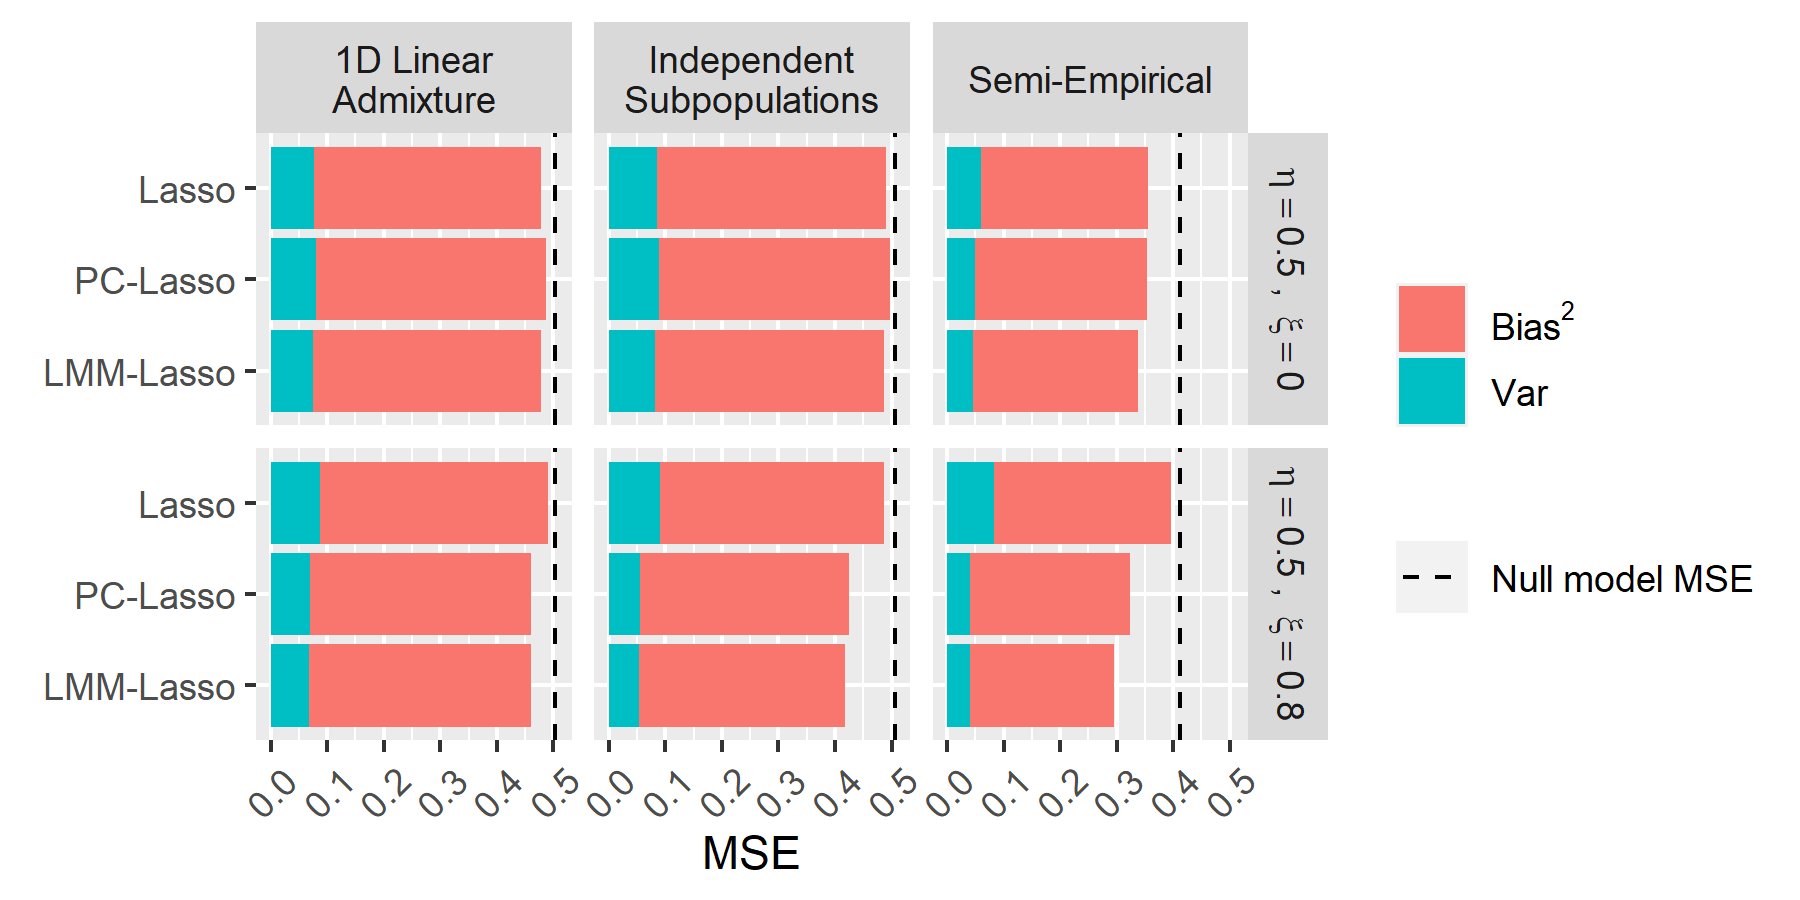
\includegraphics[scale = 1.1]{figures/beta_mse.png}
    \caption{Estimation accuracy of different methods for different data types in the presence and absence of environmental confounding with coarse subpopulation structure and dichotomous-discordant environmental effects.}
    \label{fig:mse}
\end{figure}

The bottom row of Figure \ref{fig:mse} shows the MSE when $\xi = 0.8$. In this case, both PC-Lasso and LMM-Lasso clearly outperform the ordinary Lasso. This improvement is more substantial in the Empirical and Independent Subpopulations data than in the 1D Linear Admixture data. This is due to the fact that the Independent Subpopulations and Empirical data sets are characterized by nonoverlapping genetic subpopulations, meaning that a greater proportion of the environmental effect is in the column space of $\boldsymbol{P}_{\bX}$. We can quantify the proportion of the environmental component in the column space of $\boldsymbol{P}_{\bX}$ for each data type using the CP metric defined in \eqref{eqn:ratio} of Section \ref{sec:sim_env_conf}. Here, we have CP $= 0.47, 0.99$ for the 1D Linear Admixture and Independent Subpopulations, respectively. The large CP of the Independent Subpopulations model reflects the extreme confounding and estimation bias for this data, for which the PC-Lasso and LMM-Lasso methods are able to correct. Meanwhile, the less dramatic improvement in MSE for the 1D Linear Admixture data by the PC-Lasso and LMM-Lasso methods confirms what we know from this data's substantially smaller CP value; that there is less confounding and bias which can be corrected for. 

Due to the differing sample sizes and subpopulation structures, a direct comparison of the Empirical CP $= 0.61$ with those from the simulated data sets is not straightforward. We note that the CP decreases in the presence of subpopulations of unequal sizes and with more outbred subpopulations as in the Empirical data. 

% \anna{MSPE here (?)}

% \anna{talk about karl rohe stuff here - if anywhere}

In addition to MSE, these methods' performance was also assessed in terms of variable selection using the true positive rate (TPR) for the first 50 variables each method allowed into the model. Table \ref{tab:var_sel} displays the average TPR for the same settings as in Figure \ref{fig:mse}. The TPRs echo the MSE results in that Lasso and LMM-Lasso perform comparably in the absence of environmental confounding across all data types, while the addition of the 10 unpenalized PCs leads to a slight decrease in TPR in this setting for the 1D Linear Admixture and Independent Subpopulations data sets. In the presence of environmental confounding, both LMM-Lasso and PC-Lasso achieve substantial improvements in TPR over the ordinary Lasso. As with the MSE data, these improvements are more substantial in the Independent Subpopulations and Empirical data sets than in the 1D Linear Admixture data.

\begin{table}[H]
\centering
\begin{tabularx}{400pt}{cclYYY}
\toprule
$\eta$ & $\xi$ & \multicolumn{1}{c}{Method} & 1D Linear Admixture & Independent Subpopulations & Empirical \\ 
\midrule
\multirow{6}{*}{0.5} & \multirow{3}{*}{0} & Lasso & 0.25 (0.05) & 0.23 (0.05) & 0.37 (0.06) \\ 
& & PC-Lasso & 0.23 (0.05) & 0.21 (0.05) & 0.36 (0.06) \\ 
& & LMM-Lasso & 0.25 (0.05) & 0.23 (0.05) & 0.41 (0.06) \\ 
\cmidrule{2-6}
& \multirow{3}{*}{0.8} & Lasso & 0.24 (0.05) & 0.26 (0.06) & 0.29 (0.06) \\
& & PC-Lasso & 0.28 (0.05) & 0.36 (0.06) & 0.46 (0.06) \\ 
& & LMM-Lasso & 0.28 (0.05) & 0.39 (0.06) & 0.57 (0.05) \\
\bottomrule
\end{tabularx}
\caption{True positive rates, mean (SD), for different data types in the presence and absence of environmental confounding with coarse subpopulation structure and dichotomous-discordant environmental effects.}
\label{tab:var_sel}
\end{table}

%------------------------------%
\subsection{LMM-Lasso outperforms PC-Lasso for finer population structures}
%------------------------------%

Given the superior performance of PC-Lasso and LMM-Lasso compared to the ordinary Lasso in the presence of environmental confounding, we next compare these methods in the presence of fine and coarse subpopulation structures as defined in section \ref{sec:subpopulation_structure}. Synthetic phenotypes were simulated using a 1:1 SNR, $\eta = 0.5$, and varying levels of environmental confounding, $\xi \in \{0.2, 0.5,0.8\}$. 

\begin{figure}[H]
    \centering
    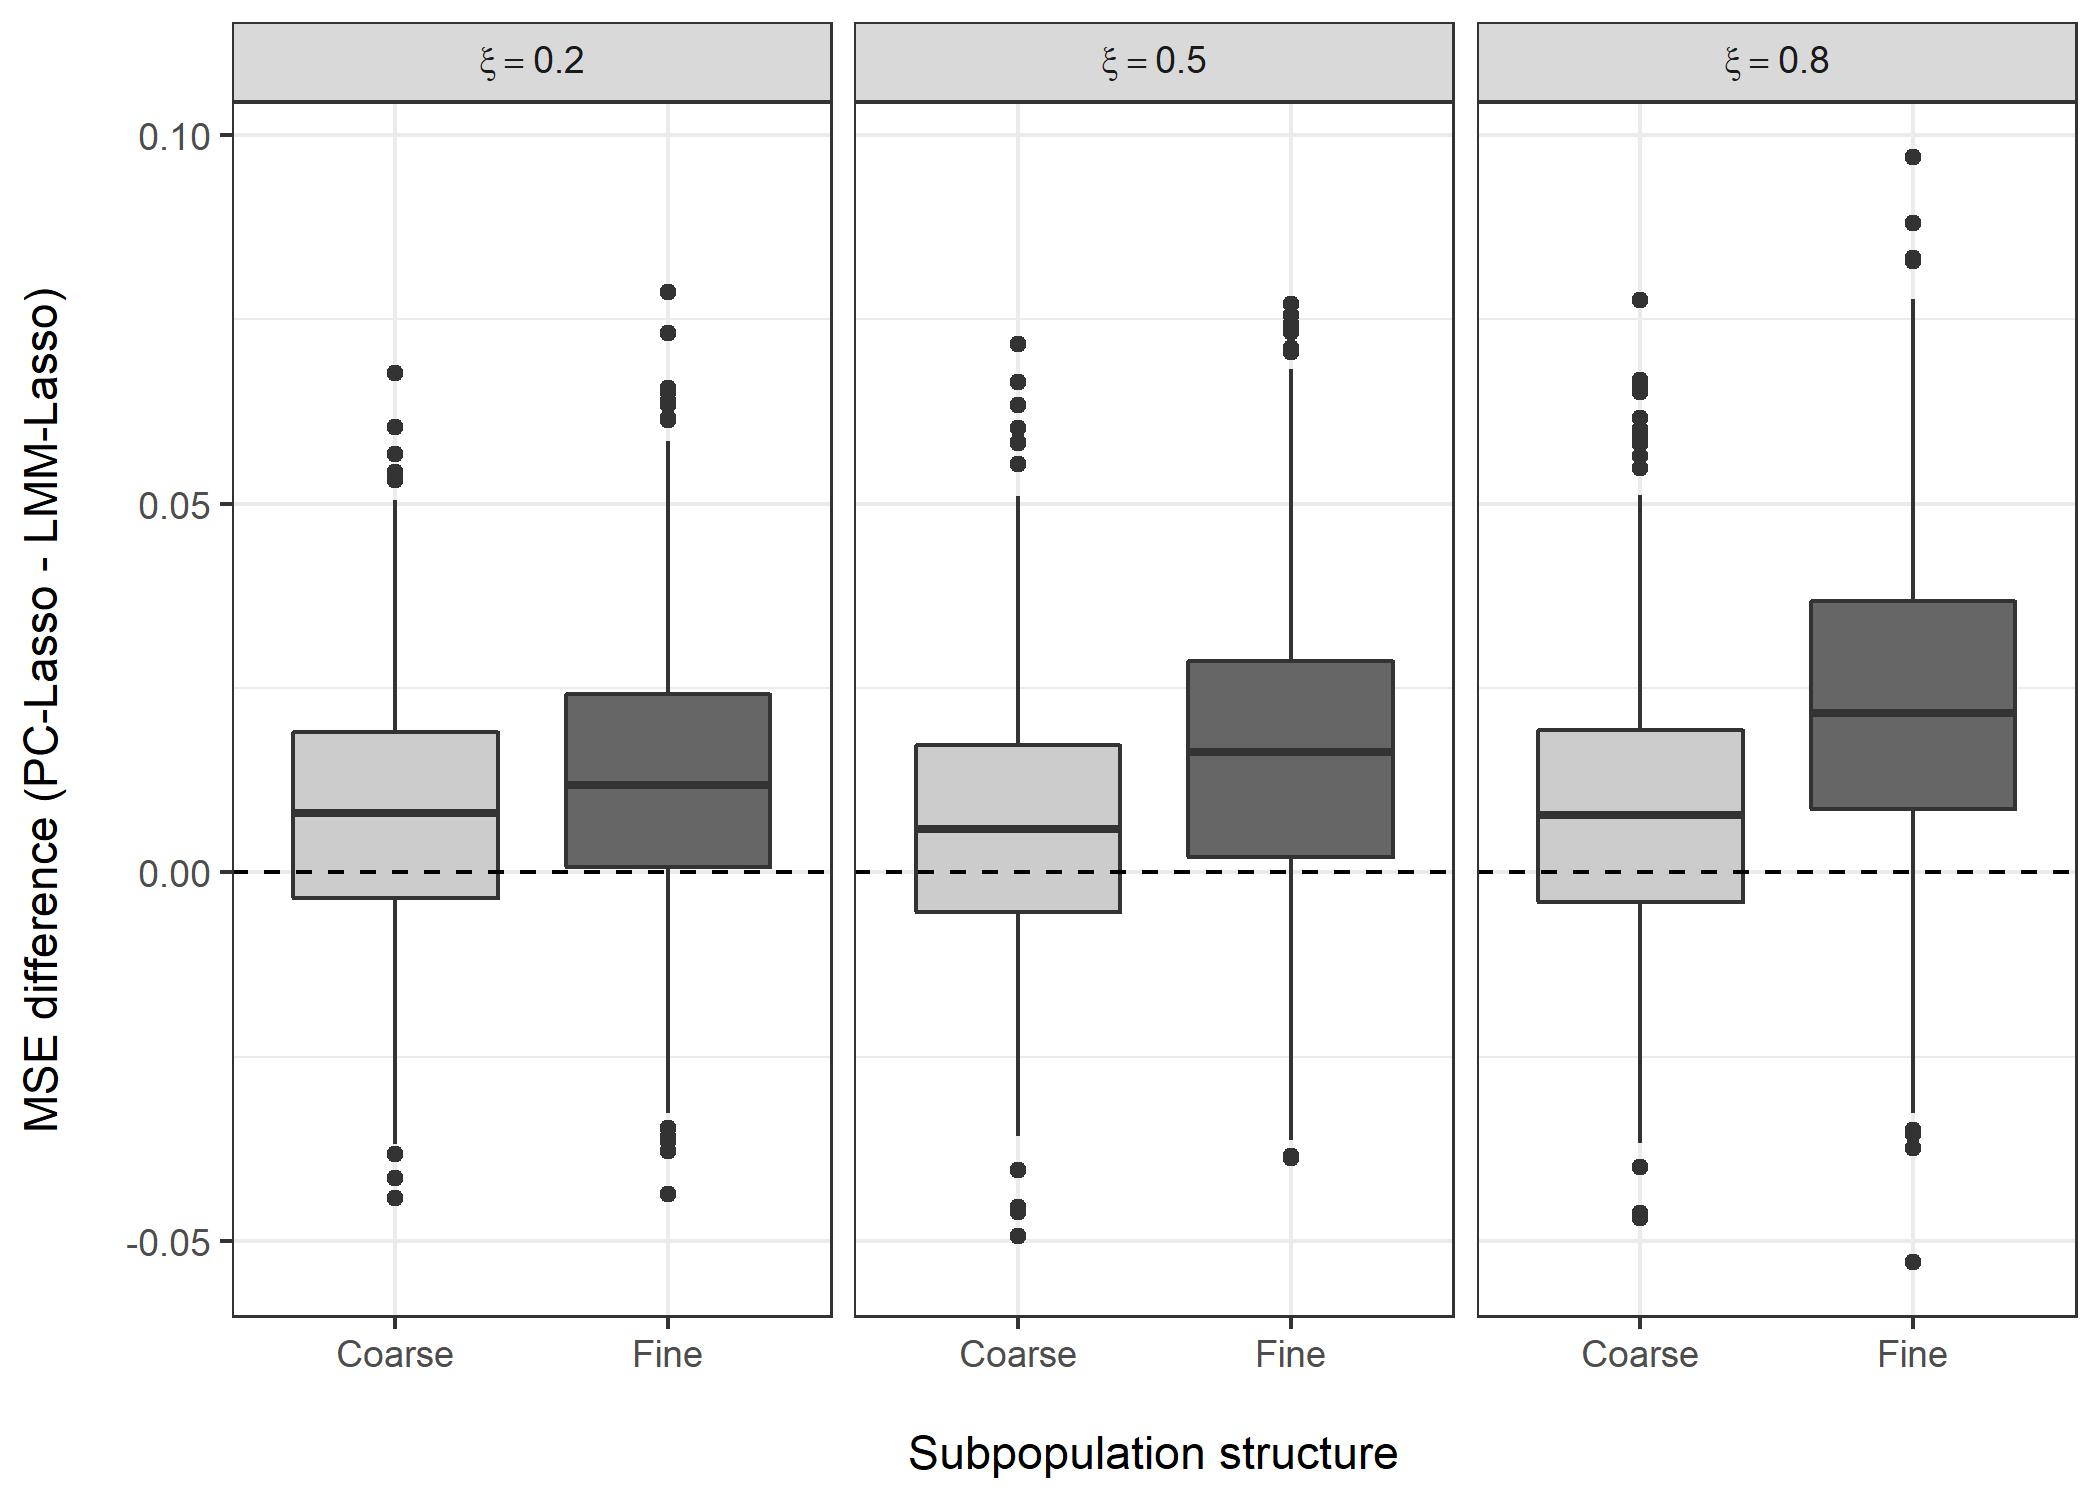
\includegraphics[scale = 0.9]{figures/mse_diff_subpops.png}
    \caption{Relative performance of LMM-Lasso, PC-Lasso for fine and coarse subpopulation structures and varying levels of environmental confounding with Independent Subpopulations data, $\eta = 0.5$, and dichotomous-discordant environmental effects. }
    \label{fig:big_vs_small}
\end{figure}

Figure \ref{fig:big_vs_small} summarizes the results of these simulations for the Independent Subpopulations and a dichotomous-discordant environmental confounding pattern, though qualitatively similar results were observed for other settings. The y-axis displays the difference in MSE (PC-Lasso - LMM-Lasso) for each simulation and for the various subpopulation structures. The dashed horizontal line at 0 indicates no difference in the performance of PC-Lasso and LMM-Lasso, while differences above 0 correspond to LMM-Lasso outperforming PC-Lasso.

Overall, in all of the settings, LMM-Lasso outperformed PC-Lasso, although the difference was considerably more pronounced when the subpopulation structure was fine.  These findings are consistent with \citet{hoffman2013correcting}, who showed that principal component adjustment methods represent a low dimensional approximation to linear mixed models. As such, it is reasonable that PC-Lasso, which corrects for population structure using a low dimensional set of surrogate variables, would perform reasonably well in the coarse subpopulation setting, but fall short in the presence of fine structure. 


%------------------------------%
\subsection{LMM-Lasso outperforms PC-Lasso when environmental effects are discordant}
%------------------------------%

In addition to evaluating PC-Lasso and LMM-Lasso in the presence of coarse and fine subpopulation structure, we also consider various patterns of environmental effects. Figure \ref{fig:big_small_gamma} shows the difference in MSE (PC-Lasso - LMM-Lasso) broken down by both subpopulation and \anna{environmental effect pattern}. Results are shown for phenotypes generated with $\eta = 0.5$, $\xi = 0.8$, and Independent Subpopulations.

% \pb{What do you think about dropping the exponential/dichotomous thing and just going with dichotomous throughout?  Doesn't really seem super important.  Well, we can just keep it in mind and if we need to cut down on space / figures, we can think about it.} \anna{so leave for now?}

The right-hand panels of Figure \ref{fig:big_small_gamma} are consistent with Figure \ref{fig:big_vs_small}, showing superior LMM-Lasso performance in the presence of fine subpopulation structure, regardless of coefficient magnitude or concordance. 

LMM-Lasso appears to perform as well, or better than, PC-Lasso in the presence of coarse subpopulation structure, as shown by the left-hand panels of Figure \ref{fig:big_small_gamma}. The upper left-hand facet in particular shows that PC-Lasso and LMM-Lasso perform more comparably when environmental effect magnitudes are exponential and concordant in nature. 
These findings align with our initial hypothesis that PC-Lasso will perform well in the presence of simple environmental effect patterns that can be well-approximated by a linear combination of the observed data. When that is not the case, either due to the presence of fine subpopulation structure, dichotomous effects, or genetic similarity that does not reflect similar environmental effects, LMM-Lasso exhibits estimation accuracy superior to that of PC-Lasso.

\begin{figure}[H]
    \centering
    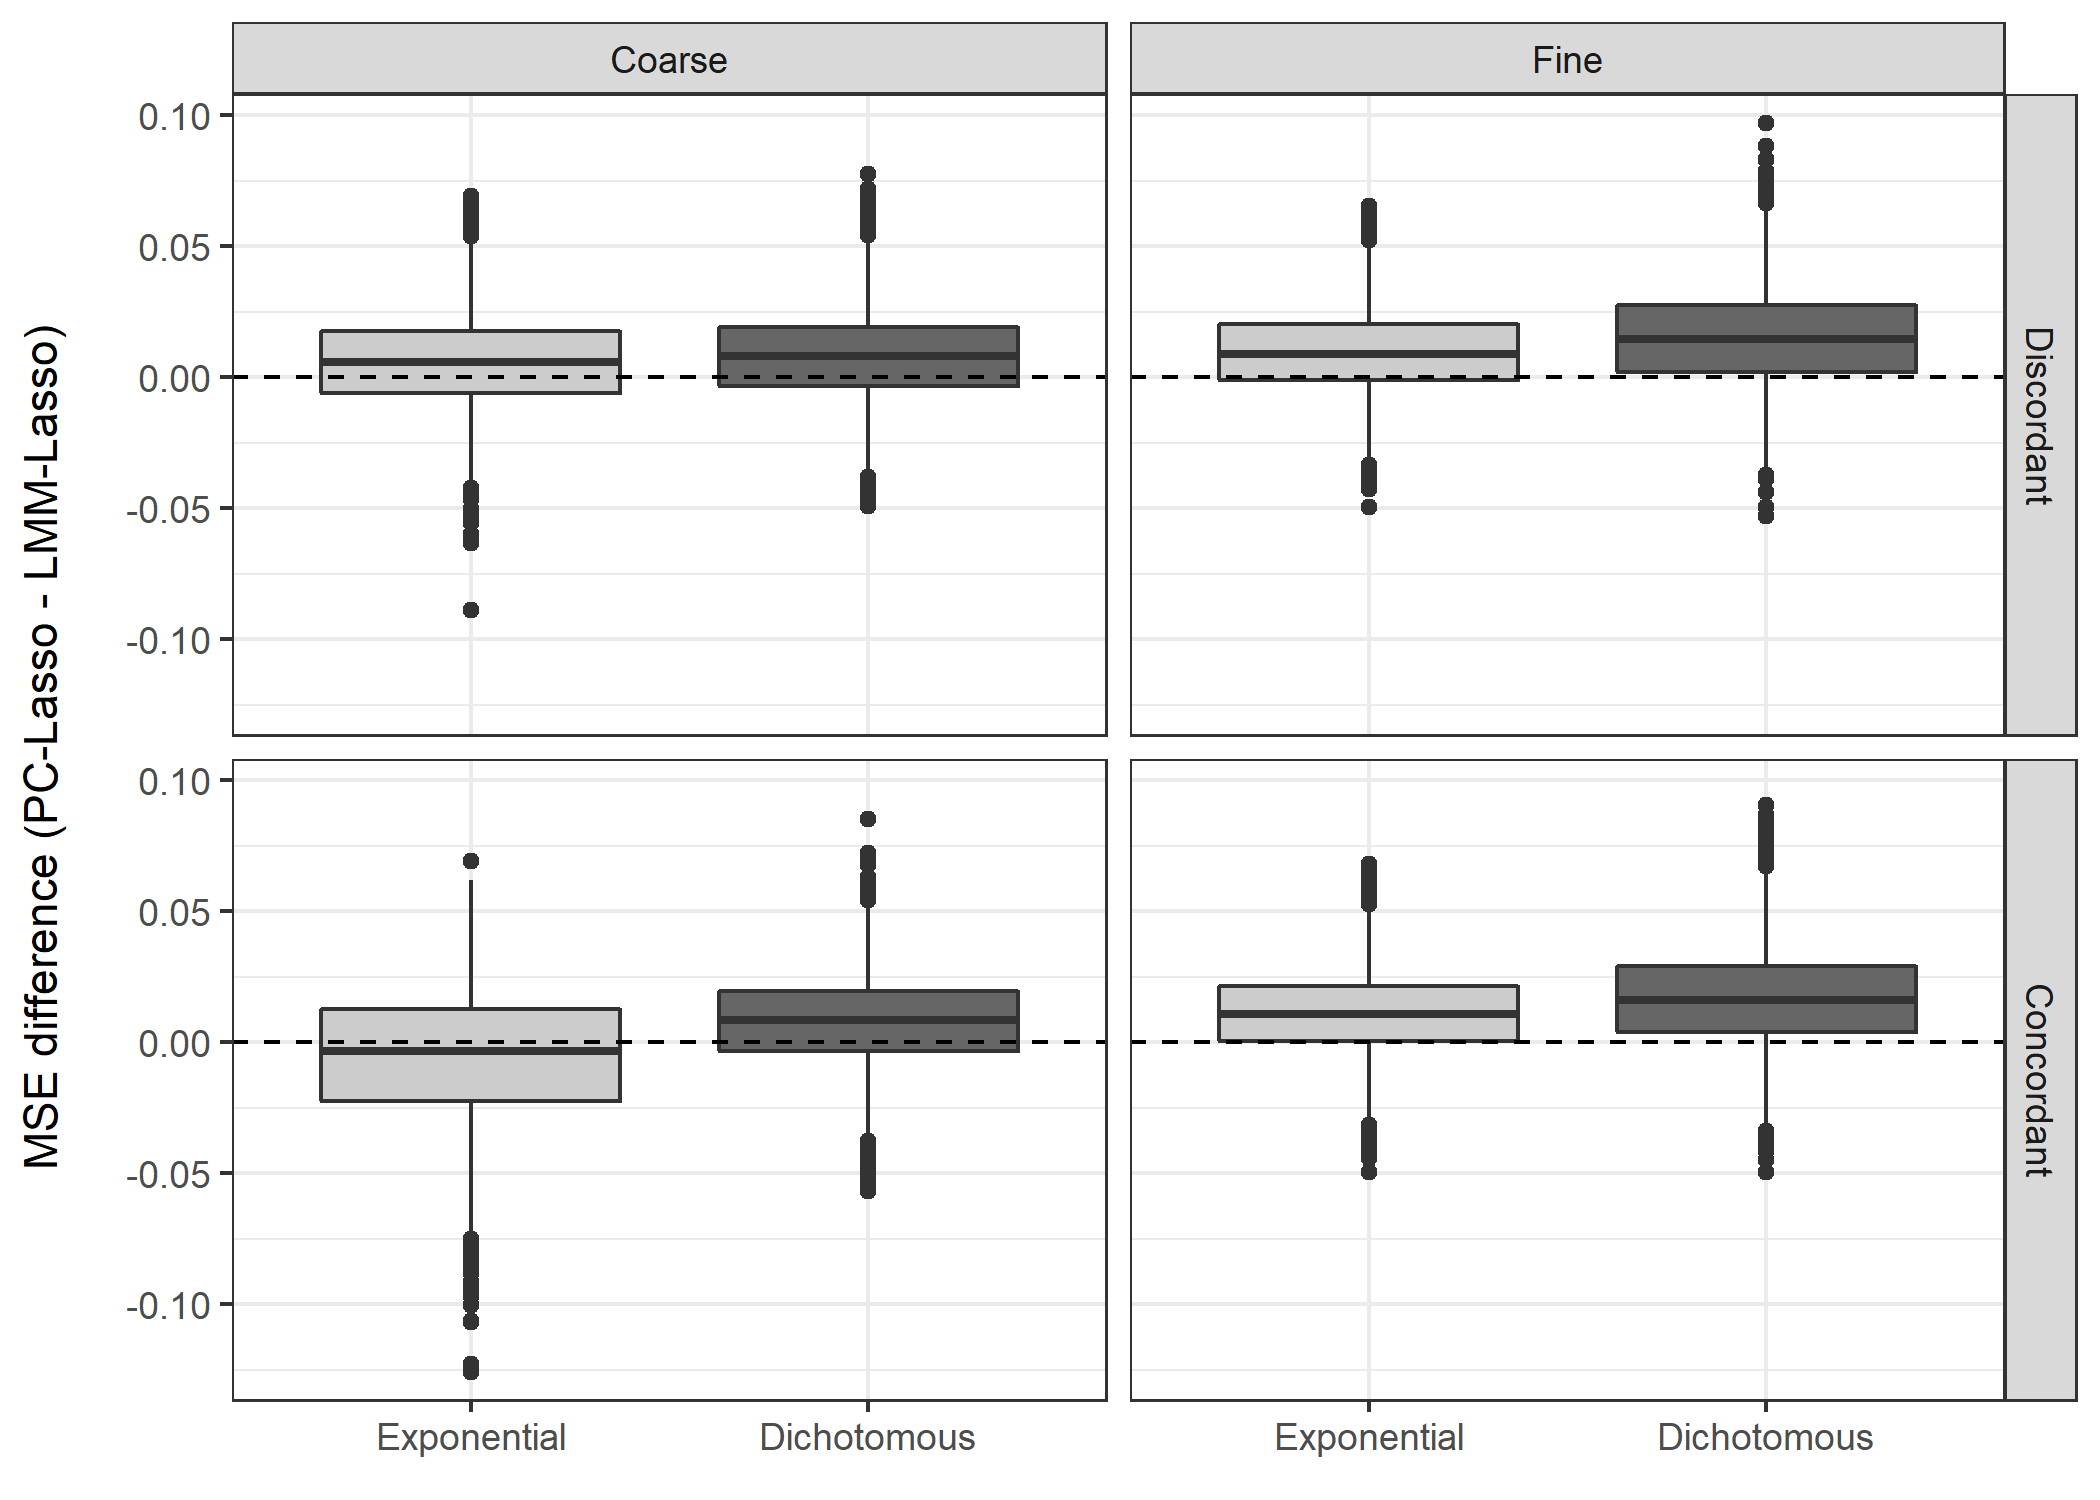
\includegraphics[scale = 0.9]{figures/mse_diff_hetero.png}
    \caption{Relative performance of LMM-Lasso, PC-Lasso for fine and coarse subpopulation structures and varying environmental effect structures with Independent Subpopulations data, $\eta = 0.5$, and $\xi = 0.8$.}
    \label{fig:big_small_gamma}
\end{figure}

%------------------------------%
\subsection{Different implementations of LMM-Lasso}
%------------------------------%

In Section \ref{sec:lmmlasso} we briefly mentioned the existence of two LMM-Lasso variants: LMM-Lasso-Rakitsch and LMM-Lasso-ggmix. Both methods perform quite similarly in terms of $\bbeta$ MSE and variable selection. Becasue of this, the preceding results, though generated using the LMM-Lasso-Rakitsch implementation, are representative of both LMM-Lasso methods in the $n = 200, p = 1000$ setting. The primary purpose of this review is to compare LMM-Lasso to other penalized regression methods with respect to correcting for population structure and environmental confounding. However, given the generally strong performance of LMM-Lasso, we also wish to discuss the key differences between these two implementations and provide guidance for potential users.

LMM-Lasso-Rakitsch uses a two-step approach. First, the variance components are estimated under the assumption of a null model. Then, the estimated variance components are used to transform the data, and the $\bbeta$ are estimated using coordinate descent. LMM-Lasso-ggmix seeks to improve upon this procedure by re-estimating the variance components and $\bbeta$ iteratively. Although this seems a reasonable approach, we have been unable to find a scenario where LMM-Lasso-ggmix reliably outperforms the LMM-Lasso-Rakitsch in estimation accuracy of $\bbeta$. In order to systematically compare both methods, we carried out simulations where $p = 1000$, $n = \{200, 400, 600, 800, 1000, 1200, 1400\}$, and $\eta = \{0.2, 0.5, 0.8\}$. Figure \ref{fig:eta_beta_mse} shows the MSE for estimation of the parameters $\bbeta$ and $\eta$, in addition to the corresponding computing time required. 

LMM-Lasso-Rakitsh and LMM-Lasso-ggmix achieve nearly identical MSE for $\bbeta$ in many scenarios, particularly where $n \ll p$, as shown in the top panel of Figure \ref{fig:eta_beta_mse}. However, when $n \ge p$ the estimation performance of LMM-ggmix becomes erratic, and in some cases worse than that of LMM-Lasso-Rakitsch. This is most dramatic in the presence of substantial environmental environmental confounding, $\xi = 0.8$, and $n = \{1200, 1400\}$. 

LMM-Lasso-ggmix achieves an improvement in the estimation of $\eta$ compared to LMM-Lasso-Rakitsch, particularly in the presence of lower $\eta$ values and where $n \ll p$, as shown in the middle panel of Figure \ref{fig:eta_beta_mse}. These improved $\eta$ estimates do not correspond to smaller $\bbeta$ MSE for LMM-Lasso-ggmix and thus do not seem to improve its estimation of the fixed genetic effects. In addition, when $n \ge 1000$, LMM-Lasso-ggmix's estimation of $\eta$ suffers. When $n \ge 1000$ and substantial environmental confounding is present, $\xi = 0.8$,  LMM-Lasso-ggmix's performance is hindered to the point that LMM-Lasso-Rakitsch estimates $\eta$ more accurately.

Overall these results show that LMM-Lasso-ggmix performs as well as LMM-Lasso-Rakitsch in estimating $\bbeta$ and outperforms LMM-Lasso-Rakitsch in estimating $\eta$ when $n \ll p$. However, these are also the settings in which LMM-Lasso-ggmix is least computationally efficient. The bottom panel of Figure \ref{fig:eta_beta_mse} shows the computing time required of each method in the various simulation settings, and shows that when $n \ll p$, LMM-Lasso-ggmix is up to 60 times slower than LMM-Lasso-Rakitsch. Conversely, in settings where $n \ge p$, LMM-Lasso-ggmix is up to 10 times faster than LMM-Lasso-Rakitsch. However, these are also settings in which LMM-Lasso Rakitsch substantially outperforms LMM-Lasso-ggmix in estimating $\bbeta$ and $\eta$ accurately and consistently. 

LMM-Lasso-ggmix's poor performance in these scenarios are likely attributable to a number of a factors such as an ill-conditioned RRM  in $n \ge p$ settings \citep{ledoit2004well}. In addition, because LMM-Lasso-ggmix attempts to estimate more parameters than LMM-Lasso-Rakitsch, its optimization problem is not necessarily convex, making it prone to getting stuck in local minima before it is able to extensively explore the coefficient path. An examination of the number of iterations required for convergence for each $\lambda$ in the coefficient path suggests that this is the case for our various simulation settings (Supplementary Figure \ref{fig:niter}). Converging to a local minimum in this manner would lead to few iterations required for each $\lambda$ value before convergence, allowing for an advantage in terms of computational speed, but poor estimation, which is what we observe in Figure \ref{fig:eta_beta_mse}.

\begin{figure}[H]
    \centering
    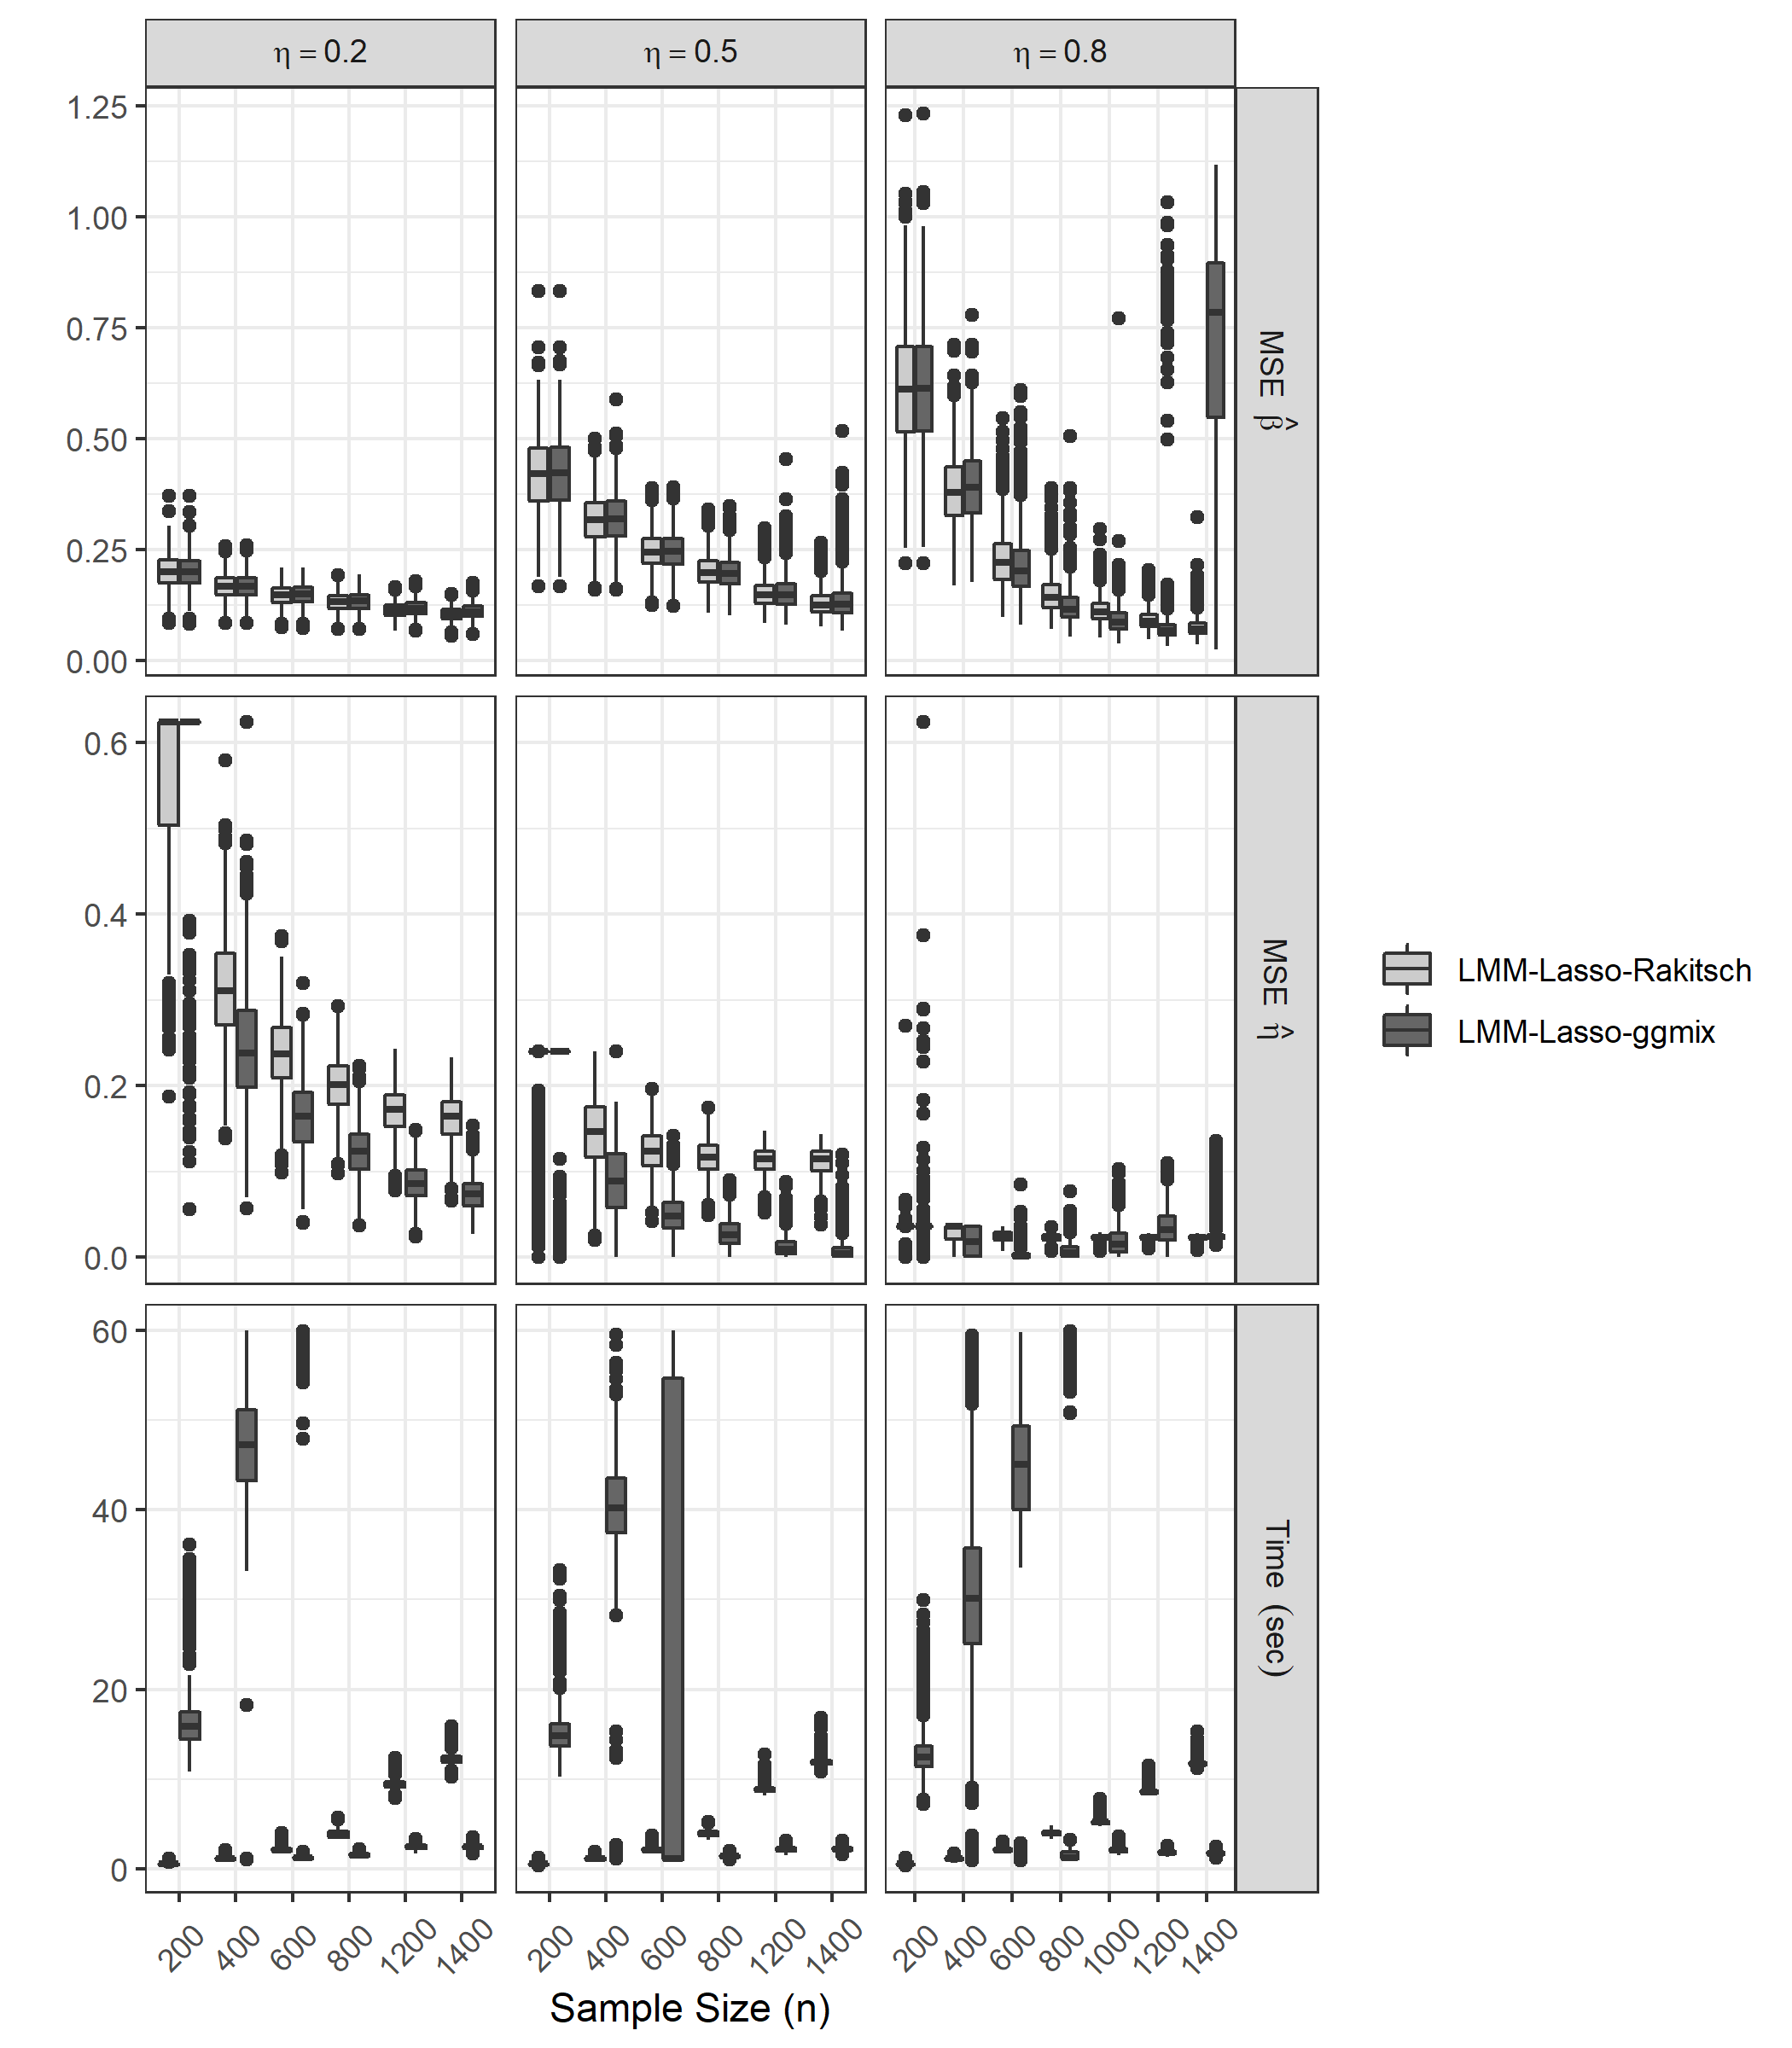
\includegraphics[scale = 1]{figures/eta_beta_hat.png}
     \caption{$\bbeta$ and $\eta$ estimation accuracy of LMM-Lasso-Rakitsch and LMM-Lasso-ggmix for varying $\eta$ levels and sample sizes with Independent Subpopulations data, coarse subpopulation structure, $\xi = 0.8$, and dichotomous-discordant environmental effect structure.}
    \label{fig:eta_beta_mse}
\end{figure}

%%%%%%%%%%%%%%%%%%%%%%%%%%%%%%%%
%------------------------------%
%%%%%%%%%%%%%%%%%%%%%%%%%%%%%%%%
\section{Discussion} \label{sec:discussion}
%%%%%%%%%%%%%%%%%%%%%%%%%%%%%%%%
%------------------------------%
%%%%%%%%%%%%%%%%%%%%%%%%%%%%%%%%

In this work, we have reviewed the concept of population stratification and explicitly defined an environmental mechanism by which it may confound the genotype-phenotype relationship \pb{not sure what this sentence means; what are you referring to?}. We have provided a broad outline of existing methods for ameliorating the effects of these unobserved confounding influences. In addition, we have provided a thorough review of two popular approaches for correcting for population structure in genetic data: PC-Lasso and LMM-Lasso. \pb{emphasize the \emph{penalized} nature of our work here, which is I think what makes it novel}

We have detailed the assumptions made by PC-Lasso and LMM-Lasso, which model confounding influences as fixed and random effects, respectively. We have also described the ways in which simulation schemes to evaluate these methods may fail to accurately capture the effects of environmental heterogeneity. In turn, we propose and utilize a simulation approach in which the estimation bias introduced by environmental heterogeneity may be evaluated. We then compare the estimation and variable selection accuracy of the ordinary Lasso, PC-Lasso, and LMM-Lasso in various confounding scenarios.

Unsurprisingly, we find that PC-Lasso and LMM-Lasso outperform the ordinary Lasso whenever environmental confounding effects are present. However, in the absence of such effects, PC-Lasso may hinder estimation accuracy and perform more poorly than even the ordinary Lasso. This is due to the fact that the principal components are unpenalized and thus included in the final model, even when they do more harm than good in explaining phenotypic variability. Additionally, we find that LMM-Lasso outperforms PC-Lasso in the presence of fine subpopulation structure and when confounding effects are discordant in nature. In the presence of coarse subpopulation structure and exponential environmental effects, PC-Lasso performs comparably to LMM-Lasso in estimation accuracy. However, LMM-Lasso is more robust to subpopulation structure and complex patterns of environmental effects. Therefore, LMM-Lasso may be a more robust method for practitioners seeking to obtain unbiased estimates when the nature of the population structure and environmental heterogeneity are unknown.  

We considered two implementations of the LMM-Lasso method: LMM-Lasso-Rakitsch and LMM-Lasso-ggmix, which differ in their variance estimation procedures and computational implementations. Although we found that both methods perform similarly in terms of $\bbeta$ estimation accuracy, LMM-Lasso-ggmix has several drawbacks. Firstly, it suffers from estimation instability in $n \ge p$ settings. Secondly, although LMM-Lasso-Rakitsch and LMM-Lasso-ggmix perform comparably when $n \ll p$, LMM-Lasso-ggmix requires up to 60 times the computing time of LMM-Lasso-Rakitsch in these settings due to its iterative estimation procedure. The additional time required of LMM-Lasso-ggmix may be worthwhile if the objective of an analysis is to accurately estimate the narrow-sense heritability in $n \ll p$ settings. However, the LMM-Lasso-Rakitsch method is more robust to varying levels of environmental confounding and sample sizes and thus more broadly applicable. 

\citet{Rakitsch2012} parameterize their model in terms of the variance components $\sigmagg$ and $\delta := \sigmaee / \sigmagg$ as previously discussed, however, we have implemented the LMM-Lasso-Rakitsch method using the equivalent but more interpretable parameterization in terms of $\eta$ and $\sigmaee$ in the \texttt{R} package, \texttt{penalizedLMM}, available on the author's github repository \url{https://github.com/areisett/penalizedLMM}.

As an additional point of interest, recall that we provide qualitative and quantitative explanations of how the degree to which differential environmental exposures may confound the genotype-phenotype relationship is dependent upon its similarity to population structure. While the objective of these explanations, and this work as a whole, is to elucidate the manner in which failing to correct for unobserved environmental effects can bias SNP effect estimates, equation \eqref{eqn:partition_e} also highlights the manner in which such unobserved and unmodeled environmental effects could lead to substantial bias in narrow-sense heritability estimates. A more detailed treatment of narrow-sense heritability estimation is beyond the scope of this paper. However, we hope this emphasizes the broad implications and importance of the subtle distinction between the effect of population structure and unobserved environmental heterogeneity. 

Finally, it is worth nothing that even in scenarios where LMM-Lasso outperforms other methods, its estimation accuracy still suffers due to the bias inherent in penalized regression methods. Because of this, bias-reduction techniques for penalized LMMs are a potentially attractive avenue for future research.
